%ब
\chapter{Results and Discussions}
 

The performance of the solutions is measured in terms of response time and
throughput while validating referential integrity in the experiments.  Response e
time and throughput are common \ac{DBMS} performance indicators.  The response
time  indicates the time taken for an operation to be completed  while
throughput measures the number of operations that can be  completed in a unit of
time. 
The performance of the operations when referential integrity validations are not
enforced is also measured and considered as the baseline with which the
solutions are compared.   Such a comparison determines the difference in
performance  when such additional validations are enforced using the \ac{API}
and provides a guideline to asses the performance impact of each solution. 

The results from the experiments are analysed and discussed in this chapter. 
Section~\ref{s:results-overview} presents an overview of the  performance of the
four solutions.  
Section~\ref{s:results-Baseline} presents the performance without referential
integrity validations.  
Sections~\ref{s:results-insert},  ~\ref{s:results-update}
and~\ref{s:results-Delete} compares the results
of all the solutions for the \texttt{insert},   \texttt{update} and
\texttt{delete} operations (respectively).   
% Section presents the analysis for the \texttt{update}
% operation for all the solutions.  
% Section discusses the results of the solutions for the
% \texttt{delete} operation.  
Section~\ref{s:comparisonOfOperations} presents an overall comparison of the
operations.  
 Finally,   Section~\ref{s:results-summary} presents a summary of this chapter.  

\newcommand{\Width}{0.5\textwidth}
\newcommand{\TB}[1]{\textbf{#1}} 

%ब 
\section{Overview of Results} \label{s:results-overview}

The experiments were performed to evaluate the response time and throughput of
the solutions in order to determine the impact of the metadata storage and
referential integrity validations on the performance of Cassandra. Notice that
the performance is measured and analysed for only the operations that trigger
referential integrity validations. That is, the response
time and throughput are measured for the \texttt{insert}, \texttt{update} and
\texttt{delete} operations across the solutions.
% The results from these experiments are presented in
% Tables~\ref{tres:ResponseTime}, ~\ref{tres:ResponsetimeRatio},
% ~\ref{tres:Throughput} and~\ref{tres:ThroughputRatio}.

The response time measures the average amount of time required to perform a
single operation on one entity. Conversely,  the throughput is the inverse of
the response time and measures the number of operations that are performed in a
unit of time. Tables~\ref{tres:ResponseTime} and~\ref{tres:Throughput} present
the mean and standard deviation of the average response time for all the
solutions and the throughput of each operation for each solution.  Notice that
the solution with the lowest response time and highest throughput has a better
performance than rest,  while the solution with the highest response time and
lowest throughput has the worst. This means that the better performing solution
can execute each operation with the least amount of time and complete more
operations in a second.



As seen in these tables,  Solution~4 performs the best amongst all since its
response times for all the  operations on every entity are the least. 
Conversely,  Solution~3 performs the worst amongst all with high response times
for all the operations and the lowest throughput in all the cases respectively. 
Regarding Solutions~1 and 2,  they perform similarly although Solution~1 is
faster with slightly smaller response times and higher throughput.  Note that
Solution~4 is slower than  Baseline  because the baseline does not perform any
referential validations or store metadata. 

% The results show the throughput and the response time of each solution to
% complete an operation with referential integrity validation on a single
% entity.  The throughput shows how many operations are performed in one second
% in each solution. 
This can be further seen in the ratios of the response time and throughput
presented in Tables~\ref{tres:ResponsetimeRatio} and~\ref{tres:ThroughputRatio}. 
The former shows the ratio of the response time of each solution when compared
to that of the baseline,  and it indicates the factor by which any solution is
slower than the baseline;  while
% many times faster or slower each solution is when compared to the baseline. 
the latter shows the ratio of the throughput when compared to that of the
baseline. 
% The results show that all the solutions perform differently and have different
% response times and throughput. 
The variations in the performance of the solutions is due to ways these store
and handle metadata.  Recall that Solutions~1 and 2 store metadata along with the
actual data where Solution~1 stores it in every row and Solution~2 stores it as
the top row of a column family.  On the other hand,  Solutions~3 and 4 store
metadata separately from the actual data  in a \texttt{Metadata} column family
but such a  \texttt{Metadata} column family is in a separate cluster in
Solution~4. 
% The results show that the way metadata is stored and retrieved in each solution
% affects its performance during validation,  when constraints are retrieved and
% used. 

From these results,  it can be seen that Solution~4  is faster than the other
solutions when performing the validations  since it caches the list of
constraints and avoids connecting to the external cluster to access the
\texttt{Metadata} column family each time  operations are invoked on entities. 
Therefore,  to locate the relevant \ac{FK} and \ac{PK} constraints of an entity, 
the constraints stored in the cache memory are re-used. 
Performance is improved significantly just by caching the 
\texttt{Metadata} column family as it reduces the number of accesses to the
column family. 

On the other hand,  Solution~3 is the slowest  because of the
way it accesses the metadata every time from \texttt{Metadata} column family. 
% of the way the metadata is accessed for the entities in this solution. 
% % irrespective of whether an entity is a parent or child the %
% \texttt{ValidationHandler} performs the same check the metedata of the entity
% % for all the solutions.  It is when this check is made it is clear if the
% entity % is a parent or child. 
% In this solution accessing
In this solution,  in order to retrieve the relevant \ac{FK} constraints for
an entity the \texttt{Metadata} column family has to be accessed.  This means
that for each operation on an entity,  an additional access is required to
\texttt{Metadata} which consumes more time. 
Moreover,  to retrieve the information about any referencing constraints within
the relevant \ac{FK} constraints of an entity,  \texttt{Metadata} is accessed
again. 
% For example,  in order to get the information of a \ac{PK} constraint stored in the
% \texttt{RConstraintName} column of a \ac{FK} constraint,  the \texttt{Metadata}
% column family is again accessed and the \ac{PK} constraint is searched.  
Thus,  in order to
complete each validation,  \texttt{Metadata} is accessed more than once. 
% \texttt{Metadata} column family has to be accessed using the connection
% object. 
Unlike Solution~4,  metadata is not cached for re-use thus costing multiple
access to \texttt{Metadata} column family. 

Meanwhile,  Solutions~1 and~2 have approximately similar response times as both
the solutions store the whole list of constraints with the actual data and 
requires no additional connections to access the relevant as well as
referenced constraints of an entity.  Note that, in Solution~1 since the constraints
are stored with each entity it performs slightly better than
Solution~2 because the latter has an additional search operation to identify the
top row in a column family to locate the relevant constraints of an entity.  Both
solutions are faster than Solution~3 mainly because these have the whole
list of constraints along with the actual data.  However,  they are slower than
Solution~4 as these have to access the constraints from each entity every time and do not
use a cache. 
% their metadata access for these solutions are easier as metadata is a part of
% the entity and no additional connection to a metadata column family is
% required. 


% Unlike this,  Solution~4 caches  metadata for entities and re-uses it thus
% saving time by not having to access a separate column family for each entity
% insertion. 

The performance of the solutions in each
operation performed on the entities is discussed in detail in the following
sections.  Notice that,  in all the tables and figures,   the
entities \texttt{Student},  \texttt{Course} and \texttt{Enrolment} are referred
to as '\texttt{s}',  '\texttt{c}' and '\texttt{e}' for the sake of brevity. 

The standard deviation of each operation is presented in the parenthesis in
Tables~\ref{tres:ResponseTime} and~\ref{tres:Throughput}. The standard deviation
measures the dispersion of the response time and throughput of an operation from
the mean. Note that in the experiments, an operation is executed over a set of
entities a 100 times, which means that one run of the experiment produces 100
values for an operation. Thus, the standard deviation measures the dispersion of
the 100 values for every operation with respect to the mean. Notice that a  low
standard deviation means that the values of the response time and throughput of
an operation is concentrated around its mean values. Conversely, a high standard
deviation means that the response time and throughput values of the operations
are widely spread. As seen from the results, Solution~4 has low standard
deviation in all the operations indicating that in all the runs of the
experiment the response time and throughput were close to the mean values. This
is because the time to access the cache is consistent and similar throughout the
operations. On the other hand, the standard deviation is always high for
Solution~3. This is because the \texttt{Metadata} column family is accessed each
time and is affected by network latency. In general, Solutions~1 and~2 have
similar standard deviations, which is lower than the standard deviation of
Solution~3 but slightly higher than Solution~4. The reason for a slightly higher
standard deviation in these solutions is because of the time consumed to



%  shows that the performance
% values of an operation in all the runs of the experiments  is concentrated
% around the mean.



%ब 
\section{Baseline Experiment} \label{s:results-Baseline}

The performance of Cassandra when referential
integrity validations are introduced  is compared with
 a baseline experiment where the operations on the entities do not trigger any
such validations.  Such a baseline serves as a reference to determine the
difference in performance of the \ac{DBMS} when validations are imposed using
the \ac{API} and to analyse the performance of the solutions. 

In the baseline experiment,  the operations on the entities represent how
operations on data are performed in Cassandra without referential integrity
validations. In order to be consistent with the solutions, the operations
\texttt{Create}, \texttt{Update} and \texttt{Delete} for the baseline are
measured in the same way it is measured for the solutions and the artificial
data for the baseline experiment is created the same way as well.
Note that, \texttt{Create} inserts all the entities for \texttt{Student},
\texttt{Course} and \texttt{Enrolment}.  \texttt{Update} performs changes on the
primary keys of \texttt{Student} and \texttt{Course} entities,  and on the
foreign keys (\texttt{CourseId}) of \texttt{Enrolment} while \texttt{Delete}
removes all the \texttt{Student},  \texttt{Course} and \texttt{Enrolment}
entities. These operations are performed precisely the same way as the
solutions, so that the comparison and analysis of results are balanced and
unbiased.

The results in terms of average response time and throughput for the baseline
experiment are presented as  bar-plots in Figure~\ref{fres:Baseline}. 
Specifically,  Figure~\ref{fres:Baseline-responsetime} shows the response time 
of each operation on a single entity in the three column families. 
Figure~\ref{fres:Baseline-throughput} presents the throughput of each operation
on the three column families in one second. 
% The analysis of the performance of each operation on an entity is discussed as
% follows. 

% 	\begin{figure}[h] \centering
% 	\includegraphics[width=. 8\textwidth]{. /figure/result/barplot-Baseline-rt.pdf}
% 		\caption{Baseline}\label{fr:Solution0-barplot}
% 	\end{figure}
	
	\begin{figure}[H]
		
		\subfigure[Response time]
		{\includegraphics[width=\Width]{figure/result/barplot-Baseline-rt.pdf}\label{fres:Baseline-responsetime}}
		\subfigure[Throughput]
		{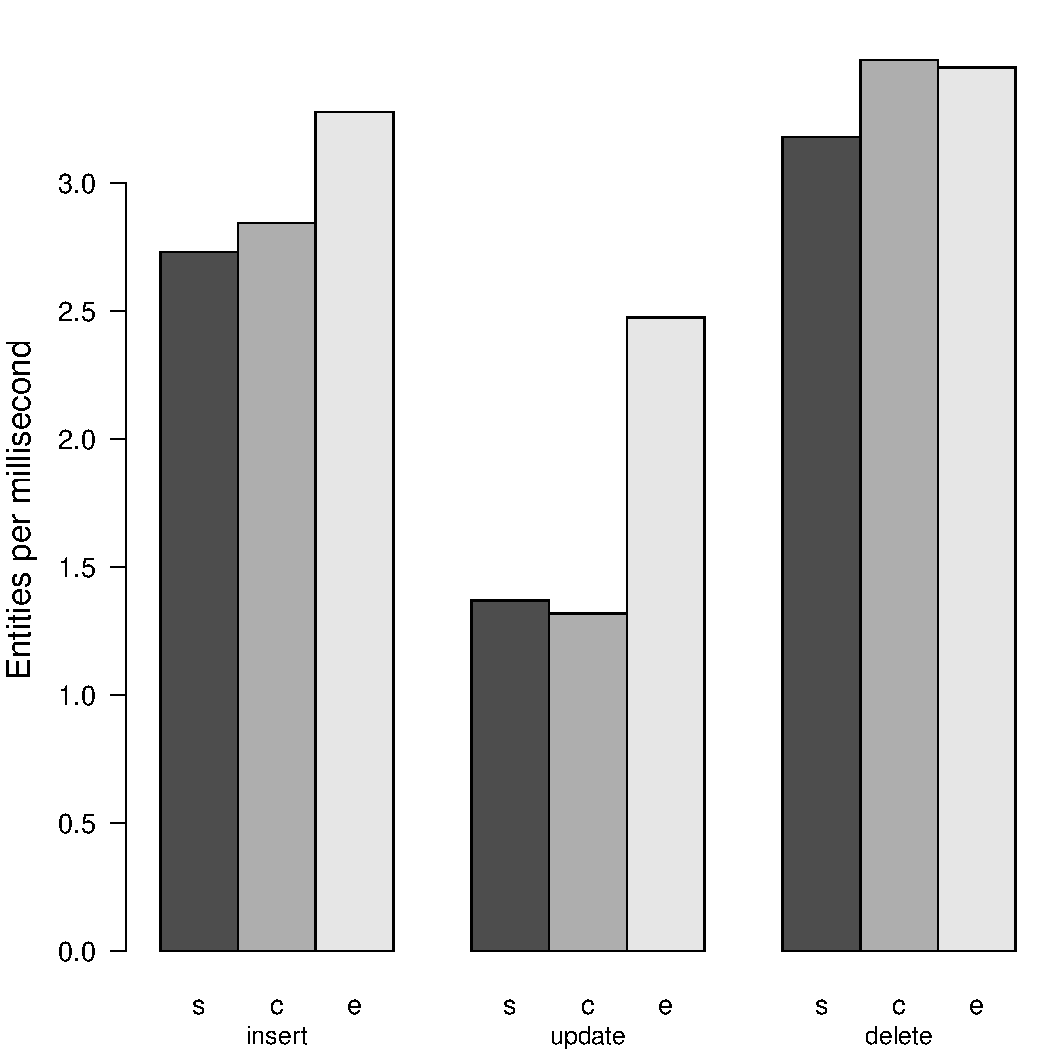
\includegraphics[width=\Width]{figure/result/barplot-Baseline-tp.pdf}\label{fres:Baseline-throughput}}
		\caption{Performance of Baseline}\label{fres:Baseline}
	\end{figure}

As seen from these results,  the \texttt{delete} operation takes in average the
least response time and  highest throughput,  respectively.  That is,  the time to
delete an entity is shorter when compared to \texttt{insert} or \texttt{update}, 
which also means that more \texttt{delete} operations can be performed within a
second.  On the other hand,  \texttt{update} takes the most time to complete all
the operations thus providing a smaller throughput while \texttt{insert} is
faster than \texttt{update} but takes slightly more time than \texttt{delete}. 

The \texttt{delete} operation performs faster than the other operations because
Cassandra performs  tombstone deletes,  where data is not physically but only
logically marked as deleted.  The \texttt{update} operation takes the most time
because it requires searching by index to access the correct columns in the
column family.  Moreover,   an \texttt{update} involves  \texttt{insert} and
\texttt{delete} operations hence takes more time that the \texttt{delete}
operation. Note that the \texttt{update} in \texttt{Enrolment} takes lesser time
because it does not change the primary keys of these entities and only the
foreign key attributes are changed.  % On the other hand,
% \texttt{update} on \texttt{Student} and \texttt{Course} entities changes the
% primary keys,  which involves performing an \texttt{insert} and a
% \texttt{delete} operation for each entity.
The \texttt{insert} operation takes slightly more time than \texttt{delete}
since data has to be physically written into the column families.

The time taken to insert one entity of \texttt{Student},  \texttt{Course} and
\texttt{Enrolment} are similar since there are no additional validations or
operations to insert these entities.  Note that the slight variations in the
perfromance for an \texttt{insert} on these entities can be due to
difference in columns,  size and external factors. 

%ब 
\section{Insert} \label{s:results-insert}
% \newcommand{\Width}{0.5\textwidth}
% \newcommand{\TB}[1]{\textbf{#1}}
% An \texttt{insert} operation triggers a referential integrity validation
% whenever a child entity containing foreign keys is inserted where the
% \texttt{ValidationHandler} validates that the foreign keys exist as primary keys
% in the parent entities.
Across all the solutions in the experiments,  \texttt{insert}  triggers a
validation when \texttt{Enrolment} entities are inserted as it is a child entity
containing foreign keys of \texttt{Student} and \texttt{Course} entities.
\texttt{Student} and \texttt{Course} entities do not trigger validations as
these do not contain any references to other column families. 

The response time and throughput for completing an \texttt{insert} on a single
entity for all the solutions are presented in Figure~\ref{fres:Insert}.
Figure~\ref{fres:Insert-responsetime} shows the time consumed by each solution
to complete one \texttt{insert} operation in each of the three entities.
Figure~\ref{fres:Insert-throughput} shows the number of \texttt{insert}
operations that can be completed in one second across the solutions.

	\begin{figure}[H] 
		\subfigure[Response time for Insert operation]
		{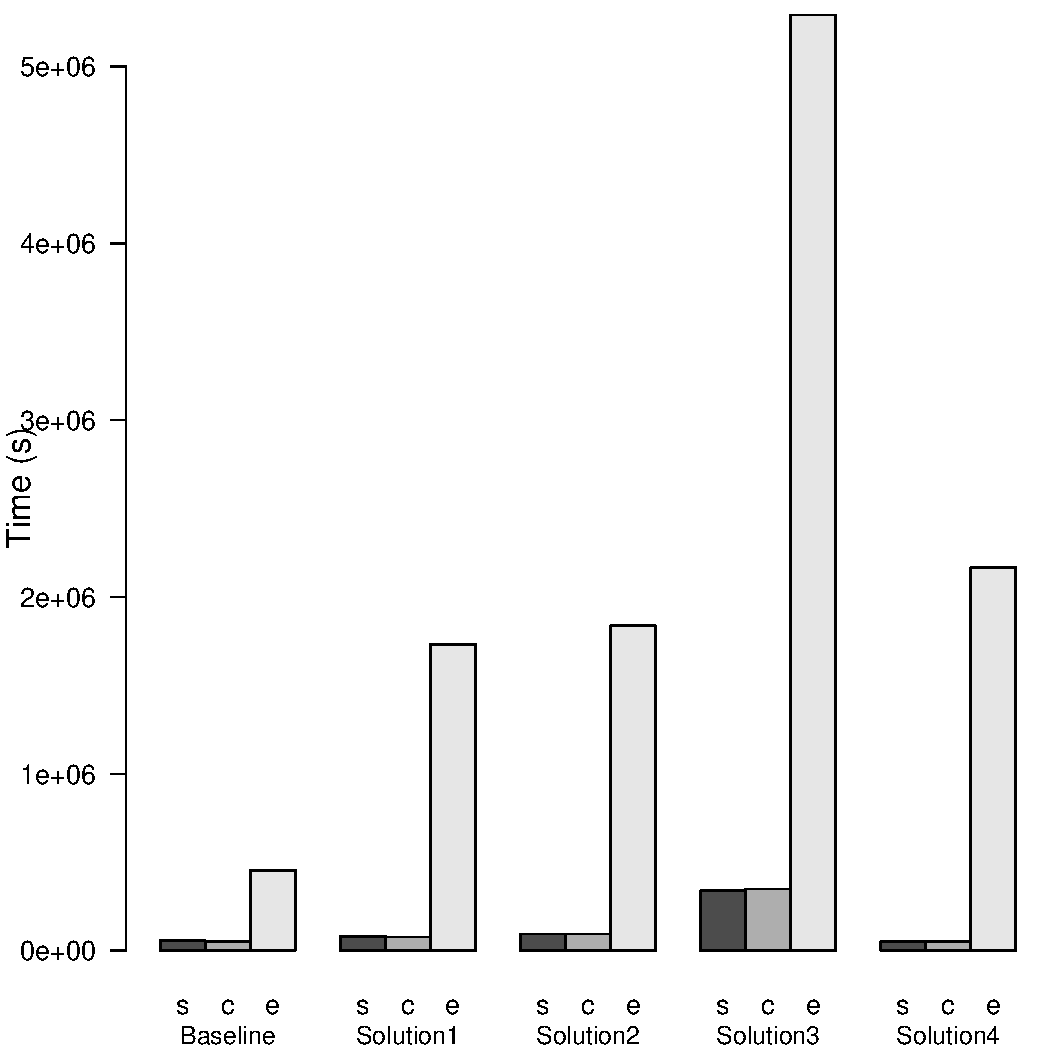
\includegraphics[width=\Width]{figure/result/barplot-insert-rt.pdf}\label{fres:Insert-responsetime}}
		\subfigure[Throughput for Insert operation]
		{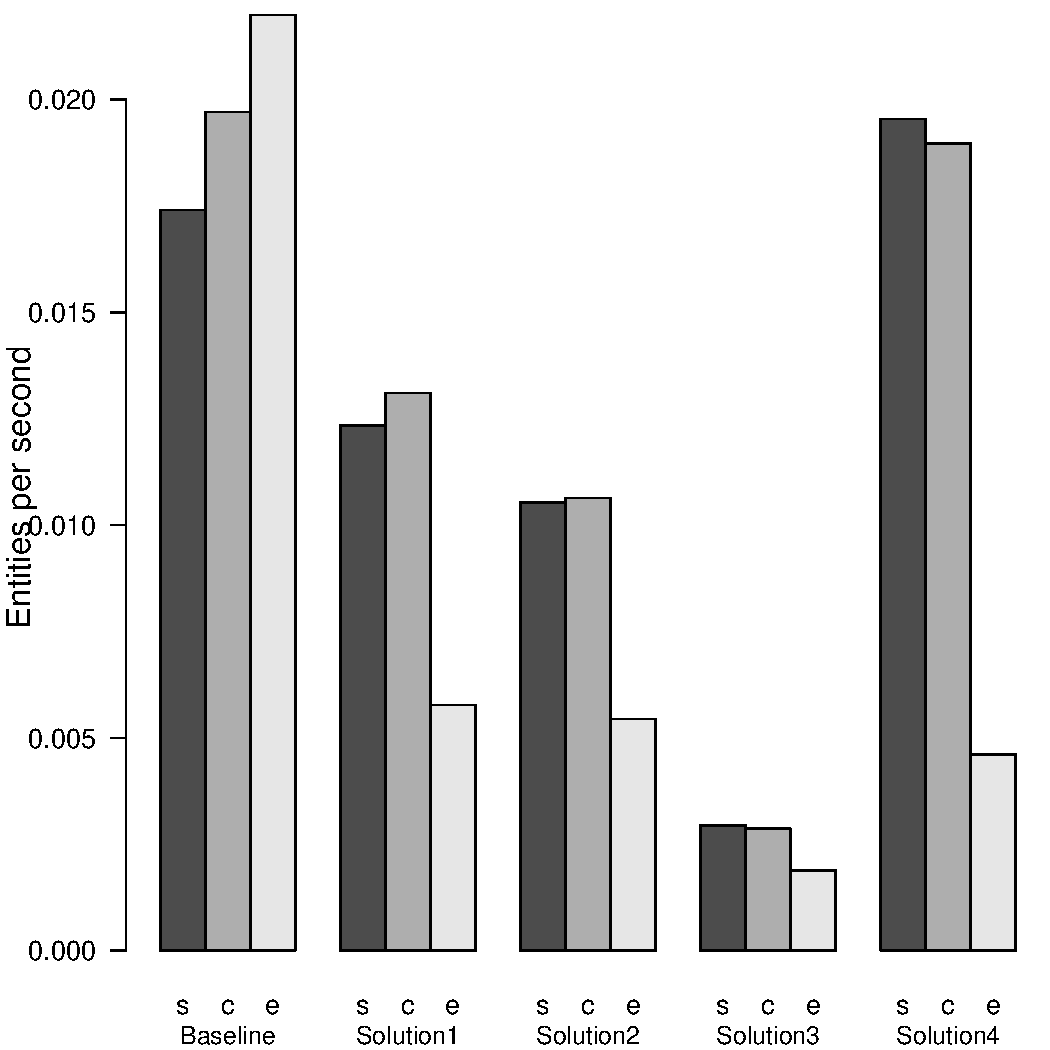
\includegraphics[width=\Width]{figure/result/barplot-insert-tp.pdf}\label{fres:Insert-throughput}}
		\caption{Performance of Solutions in Insert}\label{fres:Insert}
	\end{figure}
	
These results show
% and the results in Figures~\ref{fres:insert-user} and~\ref{fres:insert-course}
that \texttt{insert} on a single entity of \texttt{Student} and \texttt{Course}
take approximately the same time to complete. On the other hand, \texttt{insert}
on a single \texttt{Enrolment} entity takes the most time in all the solutions.
Inserting \texttt{Student} and \texttt{Course} entities into their respective
column families is fastest as these are parent column families and do not
trigger any validation. \texttt{insert} on these entities involves only
accessing its relevant \ac{FK} constraints from the metadata in order to
determine whether it is a parent or child entity. If the entity is a parent, the
validations are not triggered which is the case for \texttt{Student} and
\texttt{Course} entities. However, \texttt{Enrolment} entities have existing
\ac{FK} constraints indicating that they reference a parent entity which in turn
triggers referential integrity validations. Therefore,  its
validation involves not only identifying its relevant constraints but also
accessing its parent column families \texttt{Student} and \texttt{Course} to
ensure the existence of the foreign keys.
The results highlight the difference in response time when validation is
triggered in the case of \texttt{Enrolment} as well as when it is not initiated
in the parent entities.
% the validation of one \texttt{Enrolment} entity and for other entities that do
% not have validations.
Note that these observations stand true across all the solutions.

More information about the performance of each solution when an \texttt{insert}
operation is executed on each entity is presented in
Figures~\ref{fres:insert-user},~\ref{fres:insert-course}
and~\ref{fres:insert-enrolment}.
These figures show the response time for one \texttt{insert}
on all the three entities in every solution and the throughput for the
operations.
Figure~\ref{fres:insert-user} presents the results for \texttt{insert} on a
single \texttt{Student} entity in all the solutions. Similarly
Figures~\ref{fres:insert-course} and~\ref{fres:insert-enrolment} show the
performance of \texttt{insert} on a \texttt{Course} and \texttt{Enrolment}
entity in the solutions. It can be seen that Solution~4 takes the least time to
complete an \texttt{insert} on all the entities while Solution~3 takes the most
time. Both Solutions~1 and 2 perform similarly and are slightly slower than
Solution~4. These differences are because of the way their metadata is stored
and accessed as explained in Section~\ref{s:results-overview}.

When compared to the baseline, it is clear that the referential integrity
validations as well as metadata access caused the increased response time for
\texttt{insert} in all the solutions. Since the validations are the same for all
solutions, the performance differences in the solutions are due to the different
ways of accessing and processing the metadata.
Solution~4 is almost three times slower than the baseline to perform the
validations on \texttt{insert} while Solution~3 is more than eleven times
slower. Both Solutions~1 and 2 are almost four times slower than the baseline.
% Solution~3 takes the most time to perform one \texttt{insert} on all the
% entities.
However, when no validations are triggered Solution~4 performs almost similar to
the baseline while Solution~3 is still about two times slower than the baseline.
In this case, Solutions~1 and 2 are only about 0.5 times slower than the
baseline. Note that the time to \texttt{insert} \texttt{Student} and
\texttt{Course} entities in Baseline and Solution~4 are similar (Figures~\ref{fres:insert-user}
and~\ref{fres:insert-course}). A possible reason for this is that baseline
operations are affected by the initialization as its \texttt{insert} operations
are the very first operations to be executed.

\newpage
		\begin{figure}[H]
		\centering
		\newcommand{\W}{.4\textwidth}
			\subfigure[Response time for Insert on Student]
			{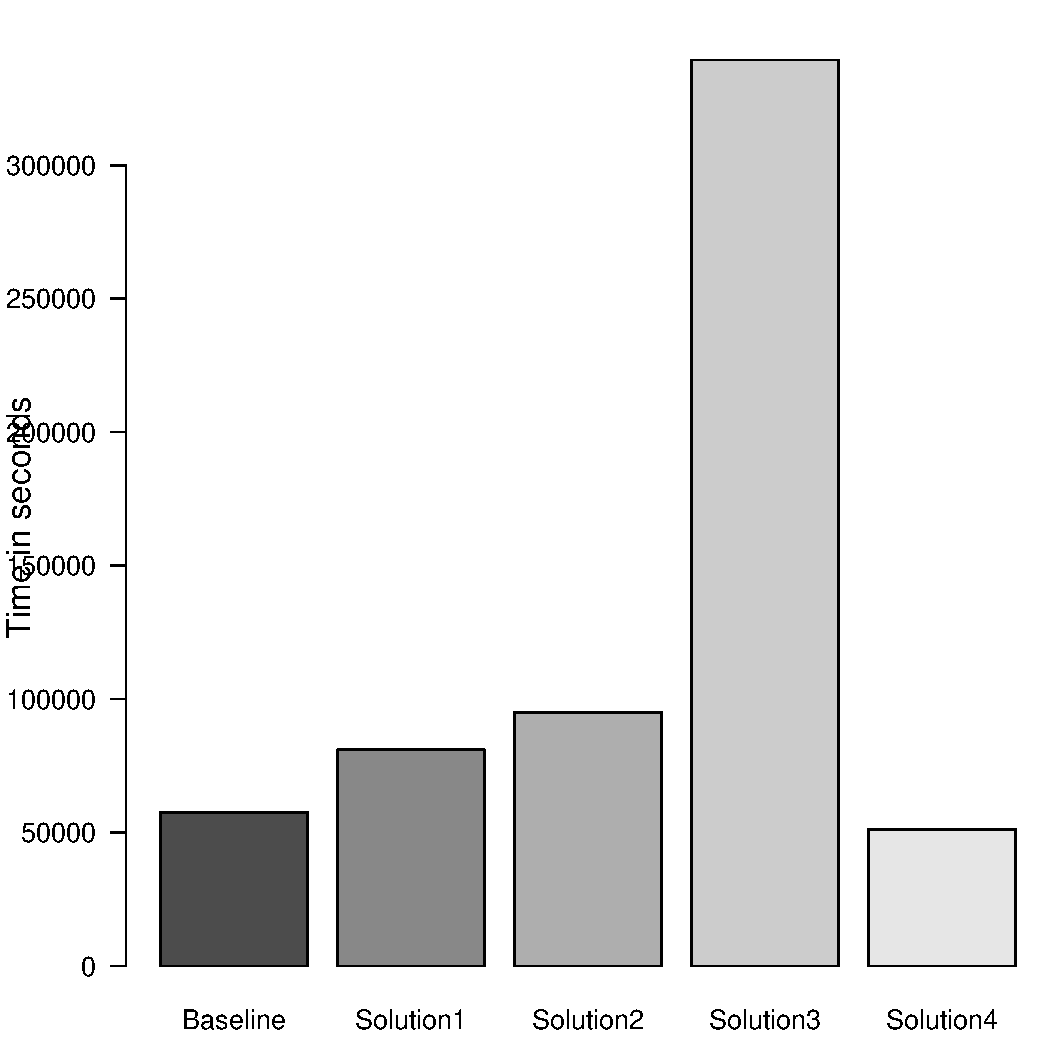
\includegraphics[width=\W]{figure/result/barplot-insert_student-rt.pdf}}
			\subfigure[Throughput for Insert on Student]
			{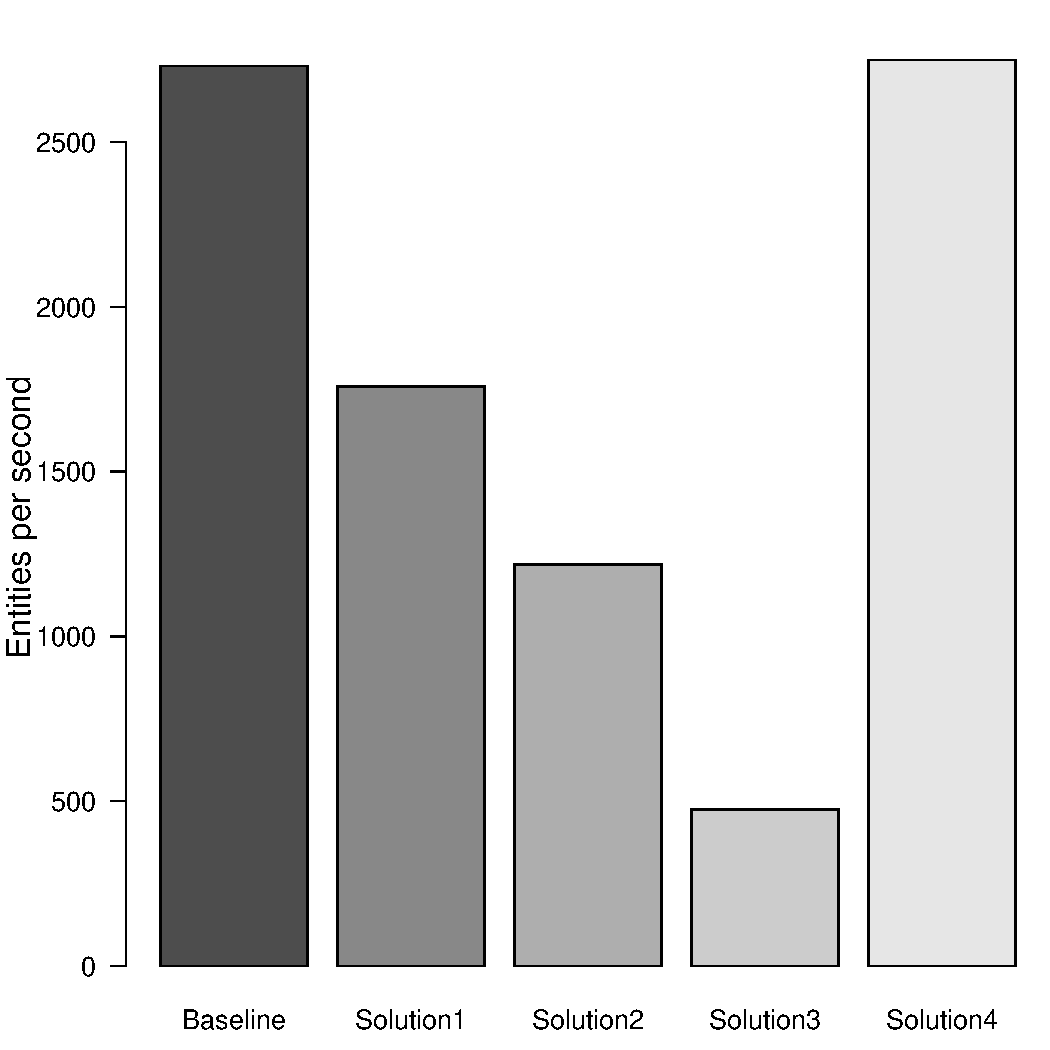
\includegraphics[width=\W]{figure/result/barplot-insert_student-tp.pdf}}
			\caption{Performance inserting students}\label{fres:insert-user}
% 		\end{figure}
% \newpage
% 	\subsection{Course}
% 		\begin{figure}[H]
			\subfigure[Response time for Insert on Course]
			{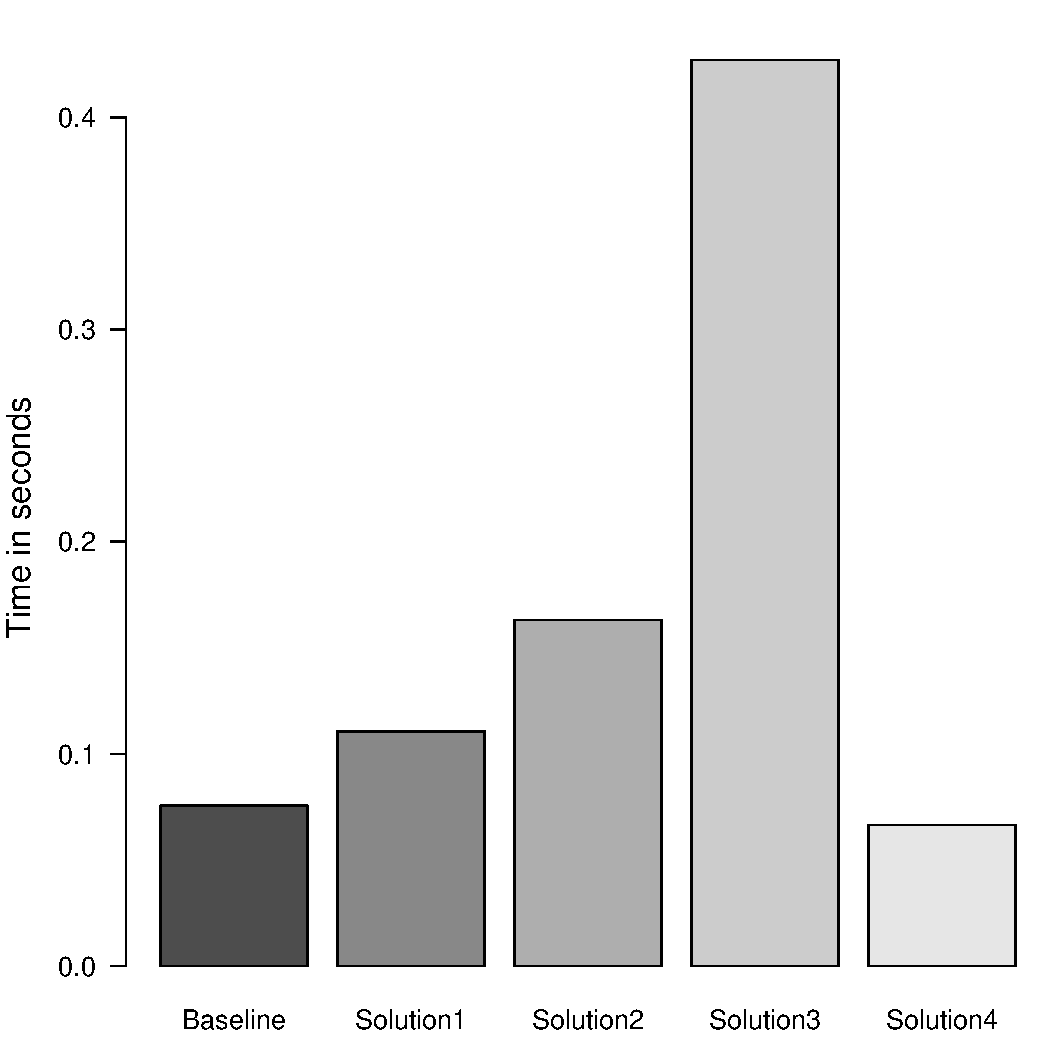
\includegraphics[width=\W]{figure/result/barplot-insert_course-rt.pdf}}
			\subfigure[Throughput for Insert on Course]
			{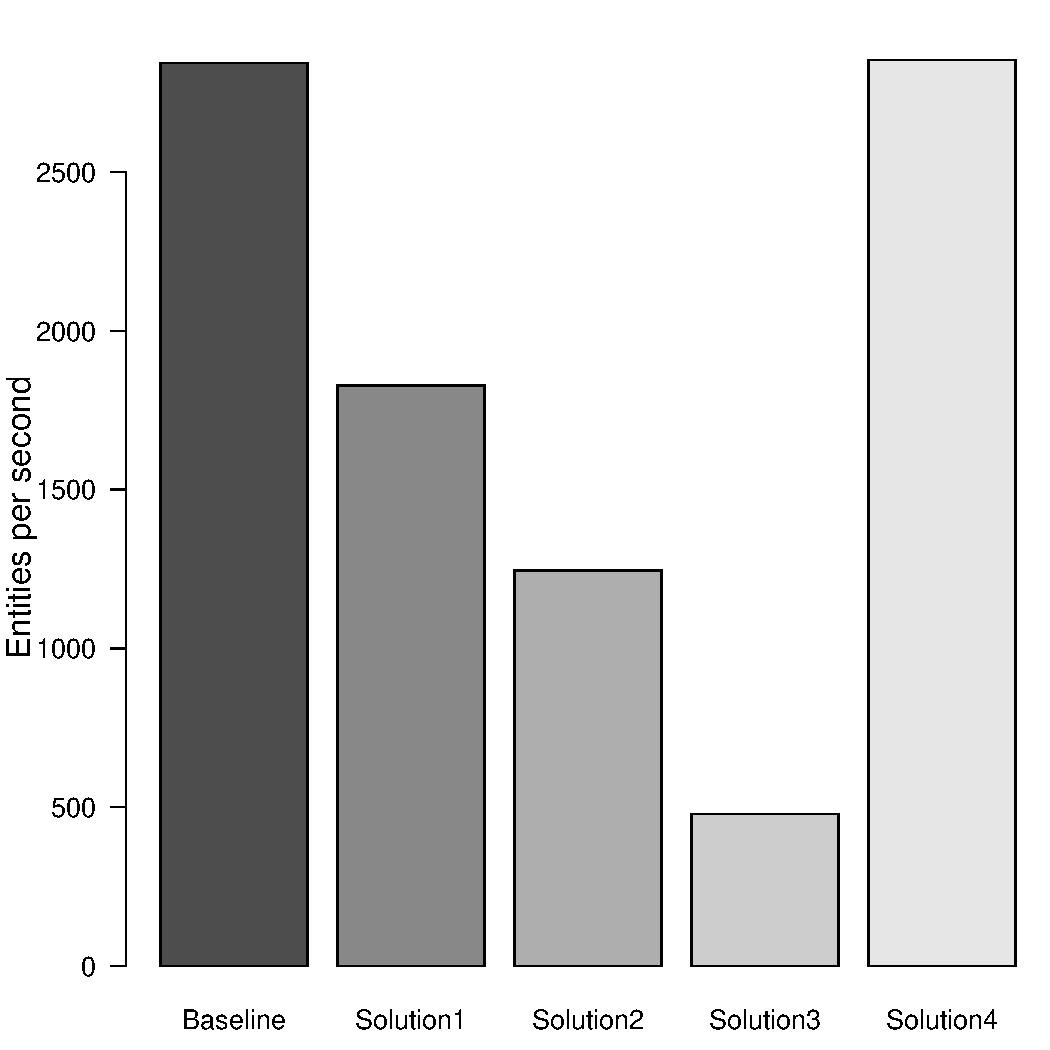
\includegraphics[width=\W]{figure/result/barplot-insert_course-tp.pdf}}
			\caption{Performance inserting courses}\label{fres:insert-course}
% 		\end{figure}
% \newpage
% 	\subsection{Enrolment}
% 		\begin{figure}[H]
			\subfigure[Response time for Insert on Enrolment]
			{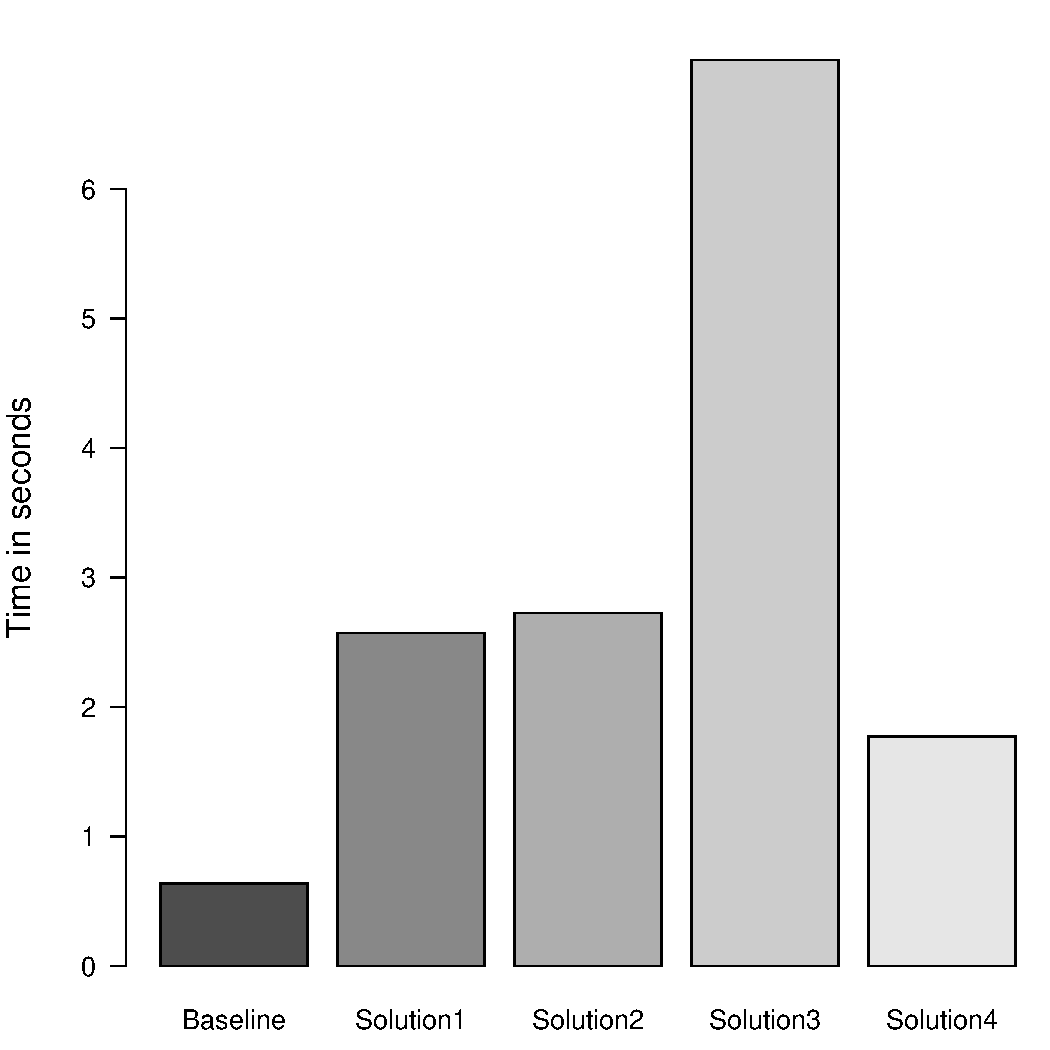
\includegraphics[width=\W]{figure/result/barplot-insert_enrolment-rt.pdf}}
			\subfigure[Throughput for Insert on Enrolment]
			{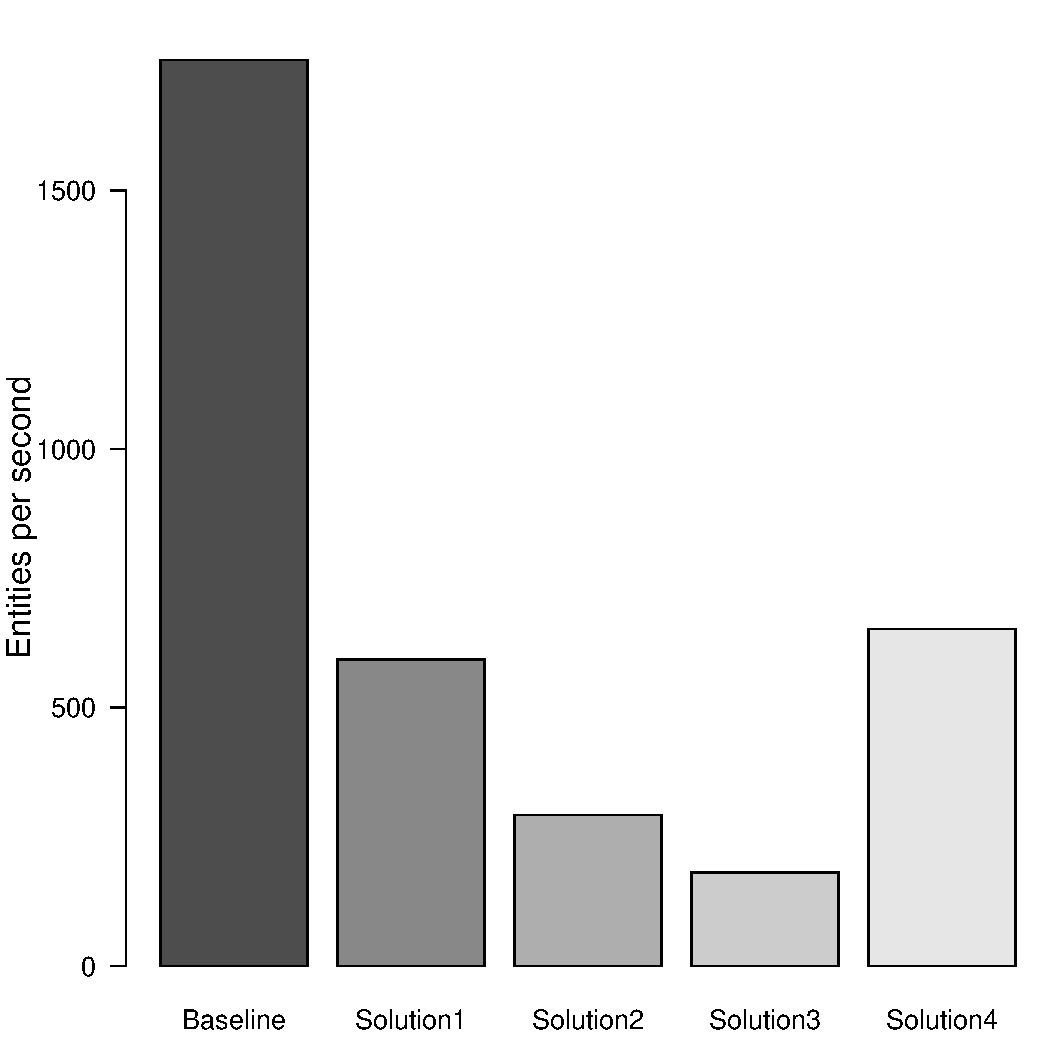
\includegraphics[width=\W]{figure/result/barplot-insert_enrolment-tp.pdf}}
			\caption{Performance inserting enrolments}\label{fres:insert-enrolment}
		\end{figure} 
%ब 

\section{Update} \label{s:results-update}
In all the solutions, the \texttt{update} operation triggers a referential
integrity validation whenever any entity of \texttt{Student}, \texttt{Course}
and \texttt{Enrolment} is updated with new values. Figure~\ref{fres:Update}
presents the results of a single update on each entity for all the solutions.
Figure~\ref{fres:Update-responsetime} shows the time taken to compete the
\texttt{update} on each entity in the solutions and
Figure~\ref{fres:Update-throughput} presents the throughput of this operation.

	\begin{figure}[H] 
		\subfigure[Response time for Update operation]
		{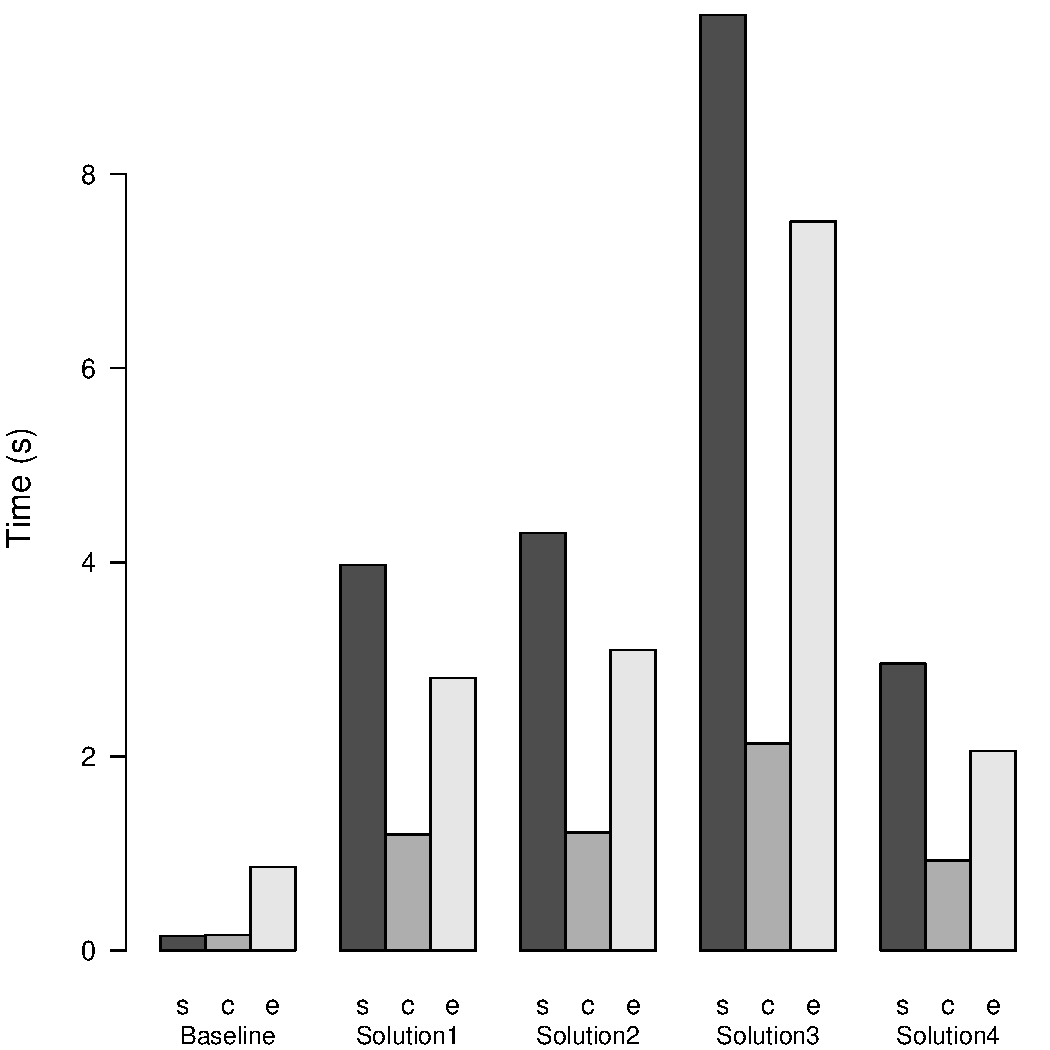
\includegraphics[width=\Width]{figure/result/barplot-update-rt.pdf}\label{fres:Update-responsetime}}
		\subfigure[Throughput for Update operation]
		{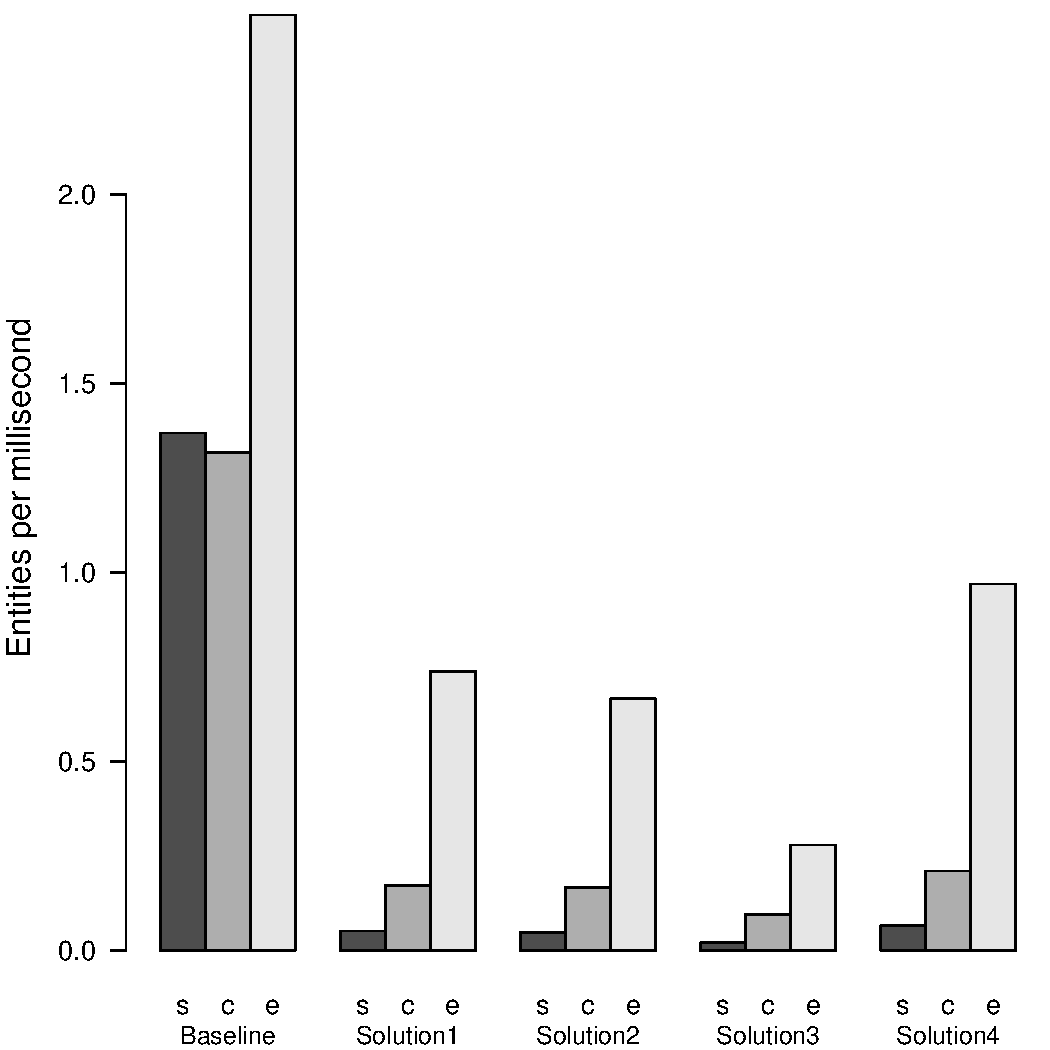
\includegraphics[width=\Width]{figure/result/barplot-update-tp.pdf}\label{fres:Update-throughput}}
		\caption{Performance of Solutions in Update}\label{fres:Update}
	\end{figure}
 
It can be seen from the results that the
\texttt{update} on \texttt{Enrolment} is the fastest in all the solutions, when
compared to \texttt{update} on other entities. On the contrary, \texttt{update}
on a \texttt{Student} entity takes the most time in all the solutions.
\texttt{update} on a \texttt{Course} entity always takes more time than
\texttt{update} on \texttt{Enrolment} but is faster than updating
\texttt{Student} entities.

These differences in the performance of an \texttt{update} on the three entities
is because of the referential integrity rules that are applied during
validation.
% which causes \texttt{update} on parent entities take more time than updating
% child entities.
Updating \texttt{Enrolment} is fastest since it involves only identifying
relevant \ac{FK} constraints in the list of constraints and then accessing the
parent column families \texttt{Student} and \texttt{Course} to verify if the new
foreign key values exist or not. After this, the new values are written to only
the \texttt{Enrolment} column family. 

However, updating a \texttt{Student} entity takes the most time since it is
a cascaded operation. After accessing its relevant \ac{FK} constraints, its
child dependencies are retrieved from \texttt{Enrolment} and updated with the new
value for the \texttt{StudentId}. This means that an \texttt{update}
accesses the metadata as well as the child column family and causes writes not
only in \texttt{Student} but also in the child column family \texttt{Enrolment}.
\texttt{update} on \texttt{Course} entities take lesser time than this because
its not a cascaded operation as the \texttt{DeleteRule} for \texttt{Course}
entities is \texttt{NoDelete}. Thus, exceptions are raised each time an
\texttt{update} is performed on \texttt{Course} entities, which means that the
response time includes measuring the time for validation as well as raising
exceptions. But this is slower than \texttt{update} on \texttt{Enrolment}
because it involves accessing the \texttt{Enrolment} column family
to identify existing child dependencies. Since these child dependencies exist
when the experiments are run, the exceptions are raised each time.

% The time involved for an \texttt{update} on a \texttt{Course} entity is  more as
% seen in Figures~\ref{fres:Update} and~\ref{fres:update-course}. In this
% operation the relevant \texttt{FK} constraints and child dependencies of the
% \texttt{Course} entity are identified and its  relevant \texttt{DeleteRule}
% is also determined.
% Since the \texttt{DeleteRule} for \texttt{Course} entities is \texttt{NoDelete}
% an exception is raised. Moreover, \texttt{Enrolment} column family is accessed
% to identify existing child dependencies. These additional operations and the
% exceptions raised make \texttt{update} on \texttt{Course} consume more time to
% complete.
% 
% The results in Figures~\ref{fres:Update} and~\ref{fres:update-user} show that
% updating a \texttt{Student} entity takes the most time in all the solutions.
% The relevant \ac{FK} constraints are accessed for this entity and
% its child dependencies are identified from \texttt{Enrolment}, which is similar
% to \texttt{update} on \texttt{course} entities. However, update on a
% \texttt{Student} entity is cascaded and involves updating all the child
% dependencies in \texttt{Enrolment} column family. This means that an
% \texttt{update} causes writes not only in \texttt{Student} but also in the child
% column family \texttt{Enrolment}. 
Note that \texttt{update} on \texttt{Student} entities causes values in
two column families to be updated, while in \texttt{Enrolment} values are
updated in only one column family and in \texttt{Course} no values are updated. 


Further details of the performance of each solution when an
\texttt{update} operation is executed on each entity is presented in 
Figures~\ref{fres:update-user},~\ref{fres:update-course}
and~\ref{fres:update-enrolment}.
% These figures show the response time to
% complete one \texttt{update} on all the three entities in every solution and
% the throughput of the operation.
Figure~\ref{fres:update-user} presents the results for an \texttt{update} on a
single \texttt{Student} entity in all the solutions and
Figures~\ref{fres:update-course} and~\ref{fres:update-enrolment} show the
performance of an \texttt{update} on a \texttt{Course} and \texttt{Enrolment}
entity in the solutions. These results show that Solution~4 is the fastest
amongst all the solutions, while Solution~3 is the slowest.
Solutions~1 and 2 perform almost similarly although the additional search for
the top row in Solution~2 makes it just slightly slower than Solution~1.
Note that in Solution~3 the \texttt{Metadata} column family is accessed multiple
times in each validation making it the slowest. Multiple accesses are needed in
order to first retrieve the relevant \ac{FK} constraints and then to retrieve
information about the child or parent entities. Although Solution~4 stores
metadata separately like Solution~3, it caches the \texttt{Metadata} column
family and reuses the cache to avoid such multiple accesses to the column
family.

When compared to the baseline, the \texttt{update} operation on all the
entities take considerably more time in all the solutions because of
their different metadata storage designs. The validations and metadata access
for parent entities make Solution~4 20 times slower than the baseline and
Solution~3 almost 60 times slower in cascaded updates, which is the most
time consuming \texttt{update}. 
Solutions~1 and 2 are almost more than 25 times slower than
baseline in such updates. However, updates on child entities make Solution~4
only slightly slower than the baseline while Solution~3 is three times slower.
In such cases, Solution~1 and 2 are almost 1.5 times slower than the baseline.

% Note that in all the solutions the \texttt{update} on . This is because of the different
% referential integrity rules applied on the entities. 
 
\begin{landscape}
		\begin{figure}
		\centering
		\newcommand{\W}{.4\textwidth}
			\subfigure[ Update on Student]
			{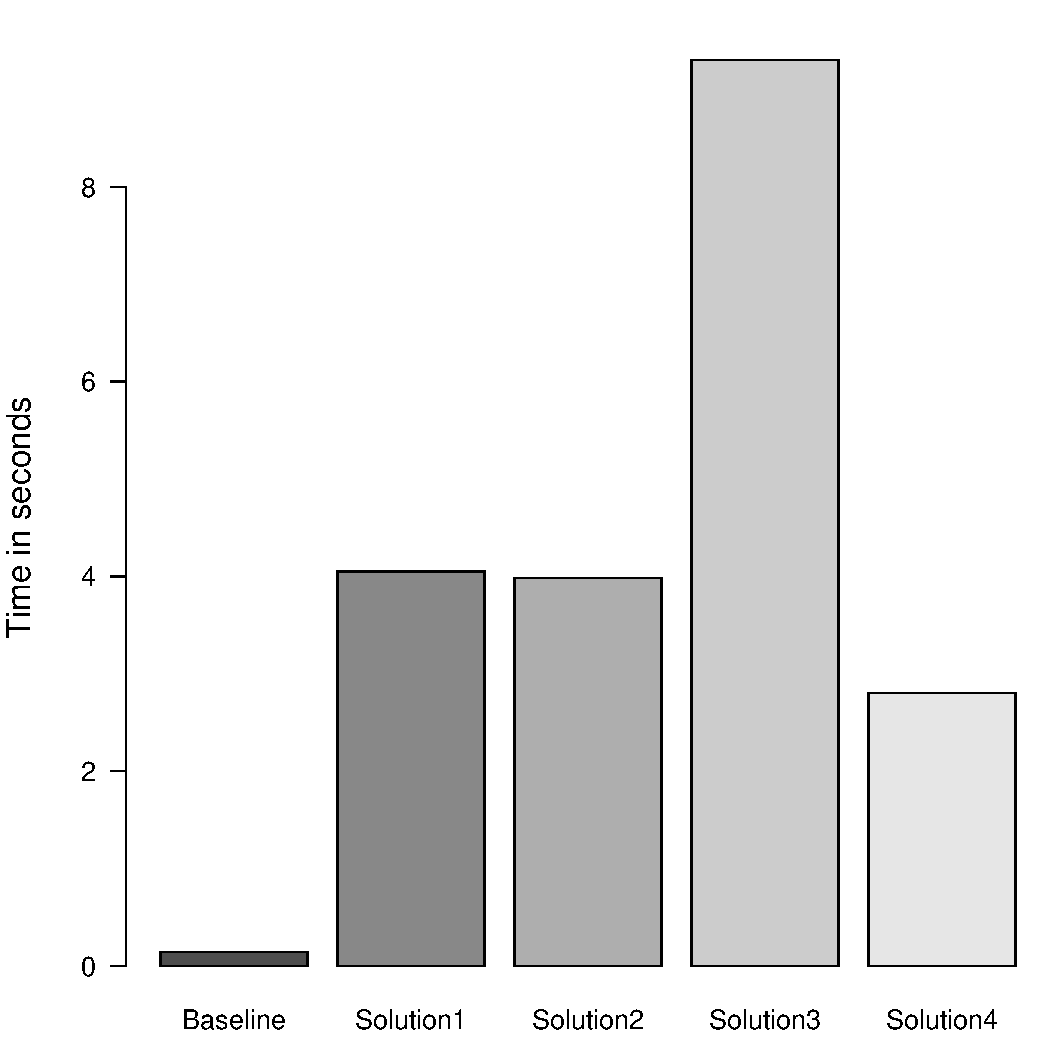
\includegraphics[width=\W]{figure/result/barplot-update_student-rt.pdf}}
			\subfigure[ Update on Course]
			{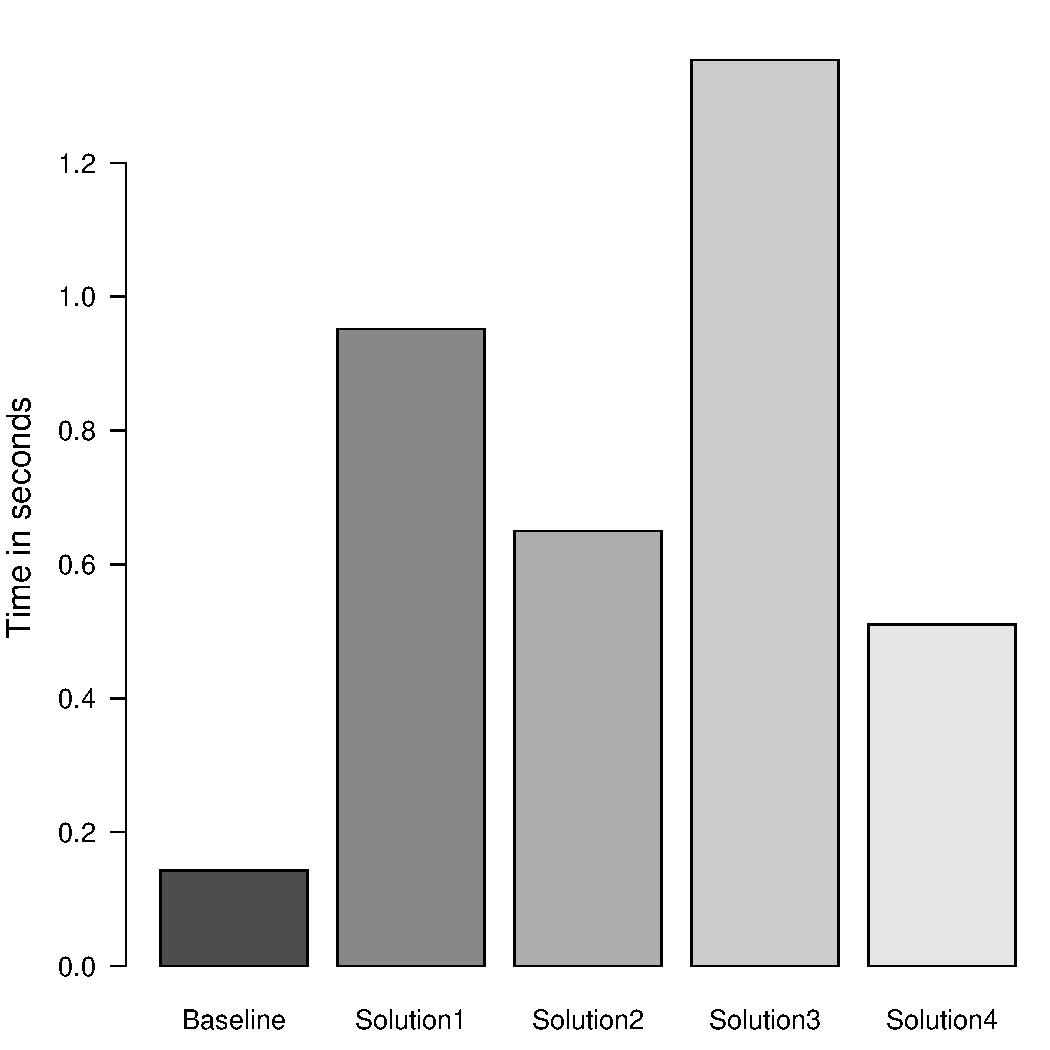
\includegraphics[width=\W]{figure/result/barplot-update_course-rt.pdf}}
			\subfigure[ Update on Enrolment]
			{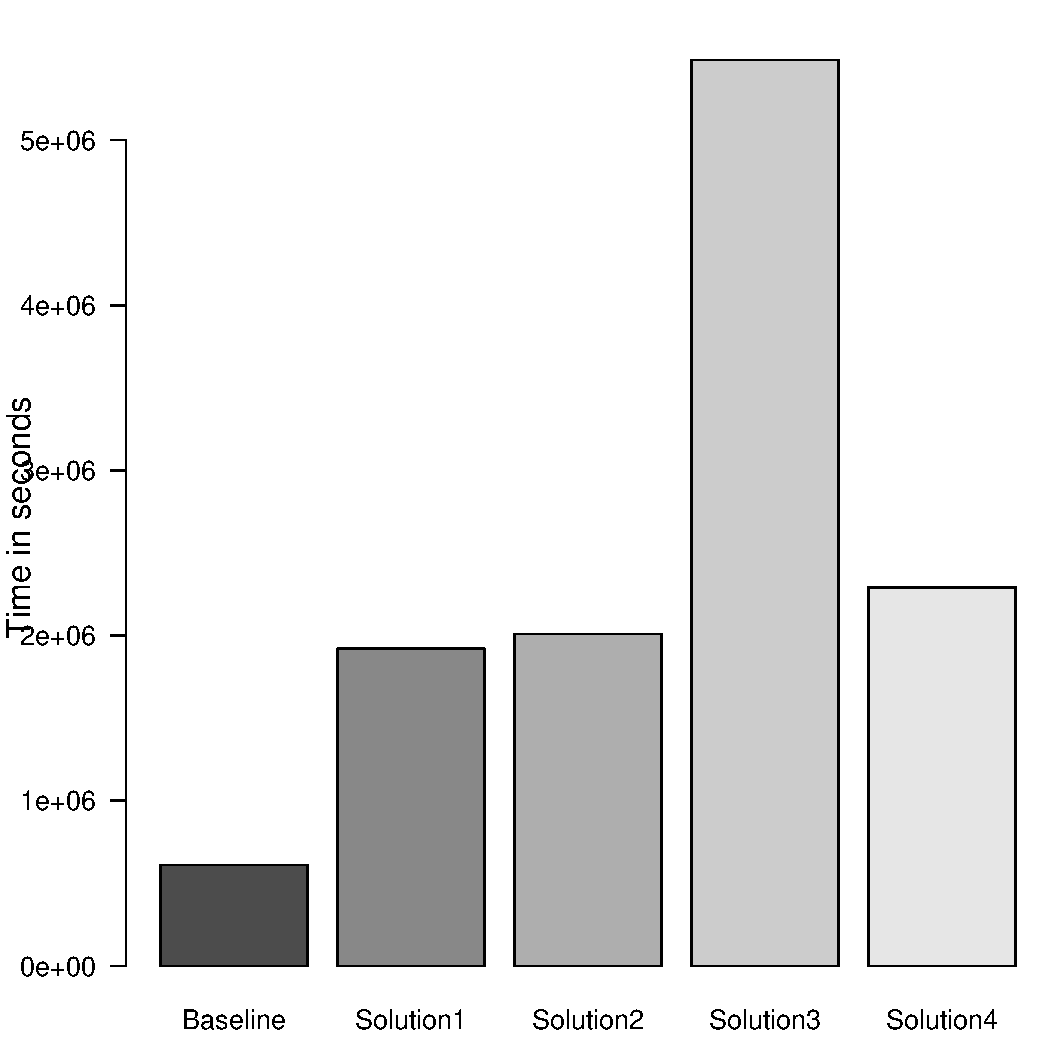
\includegraphics[width=\W]{figure/result/barplot-update_enrolment-rt.pdf}}
			\caption{Response time updating entities}\label{fres:update-response-time}
			
			\subfigure[Update on Student]
			{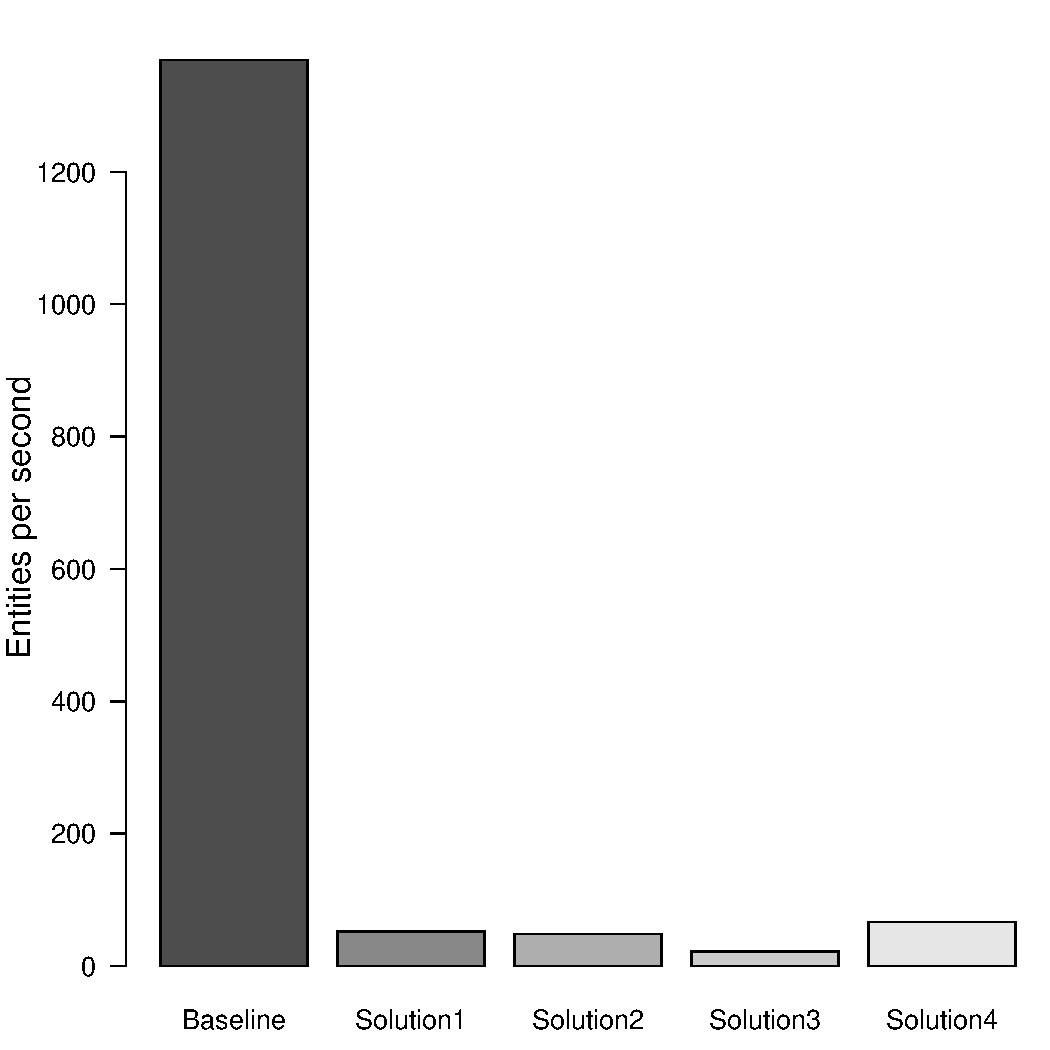
\includegraphics[width=\W]{figure/result/barplot-update_student-tp.pdf}}			
			\subfigure[ Update on Course]
			{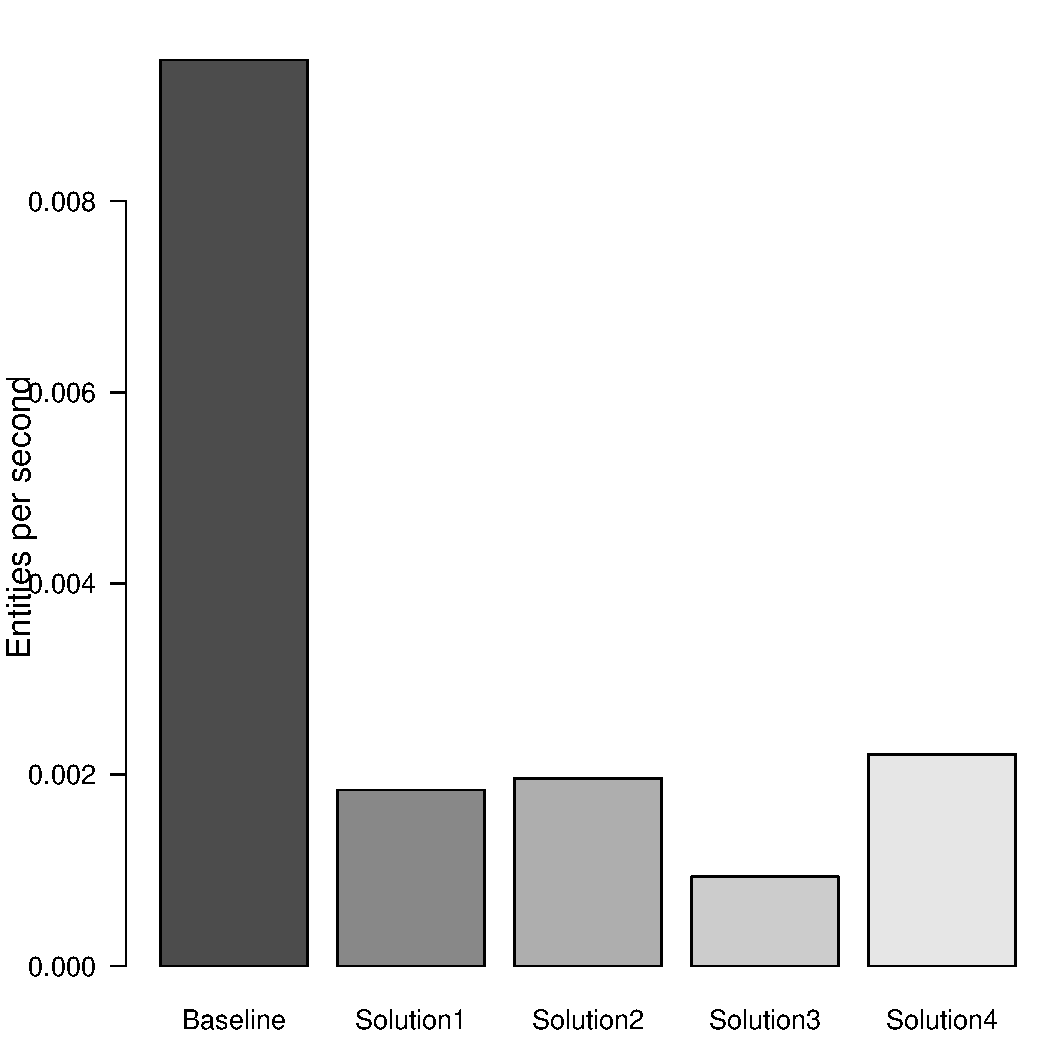
\includegraphics[width=\W]{figure/result/barplot-update_course-tp.pdf}}
			\subfigure[Update on Enrolment]
			{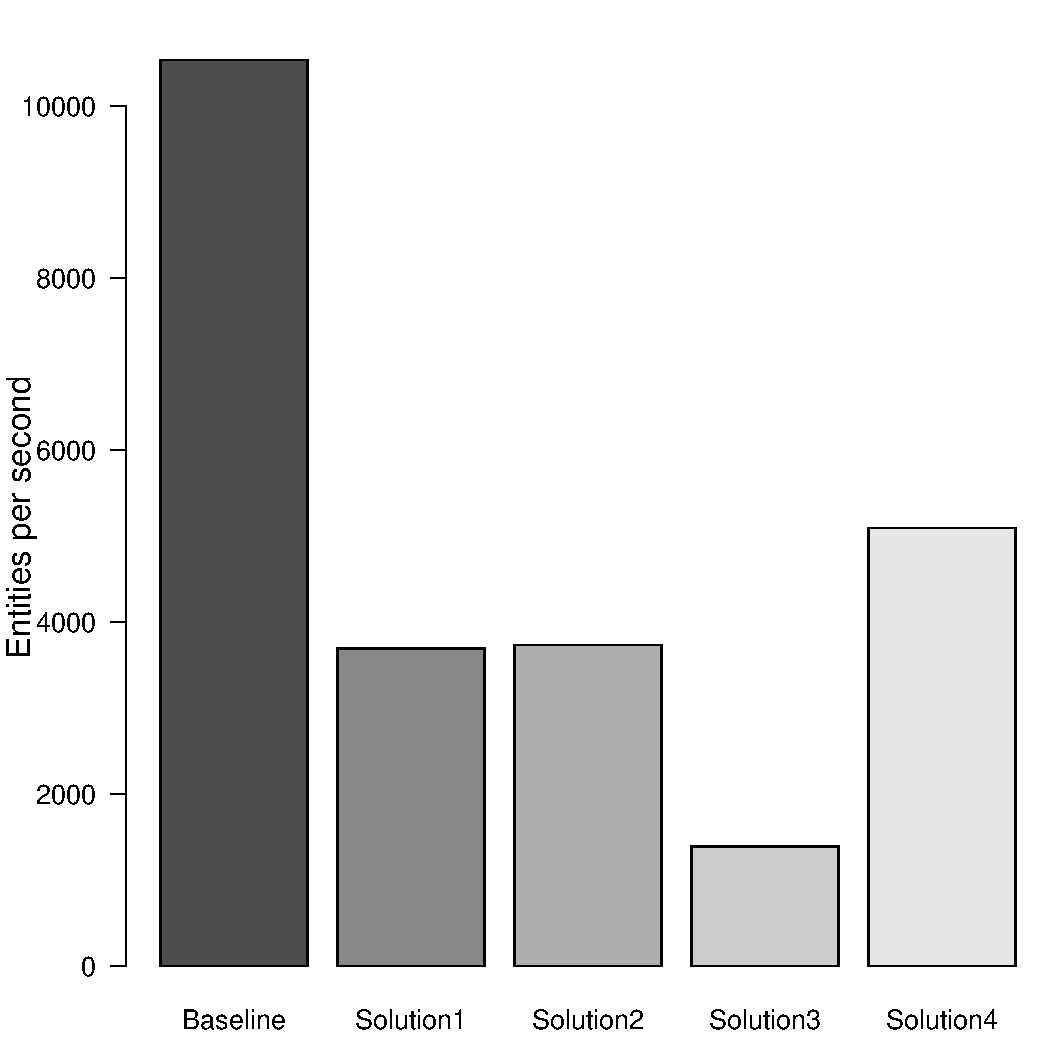
\includegraphics[width=\W]{figure/result/barplot-update_enrolment-tp.pdf}}
			\caption{Throughput updating entities}\label{fres:update-throughput}
		\end{figure}
\end{landscape}
%ब 
\section{Delete} \label{s:results-Delete}

The \texttt{delete} operation triggers referential integrity validations
whenever entities are deleted in the experiments.
Figure~\ref{fres:Delete} presents the results of the \texttt{delete} operation
on each entity for all the solutions.
Specifically, Figure~\ref{fres:Delete-responsetime} shows the average
response time to perform a single \texttt{delete} on each entity in the
solutions and Figure~\ref{fres:Delete-throughput} presents the
respective throughput for this operation.

	\begin{figure}[H] 
	\newcommand{\W}{.5\textwidth}
		\subfigure[Response time for Update operation]
		{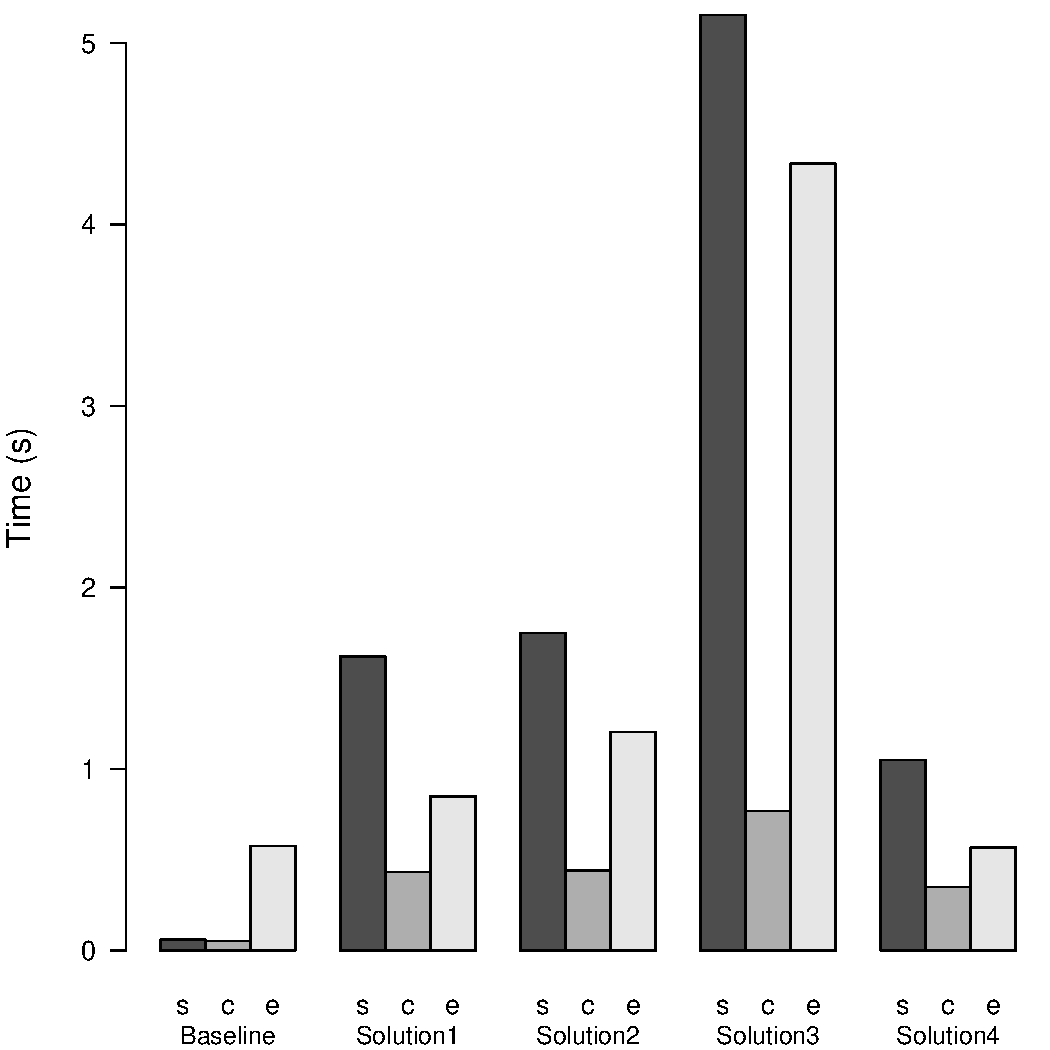
\includegraphics[width=\W]{figure/result/barplot-delete-rt.pdf} \label{fres:delete-}\label{fres:Delete-responsetime}}
		\subfigure[Throughput for Update operation]
		{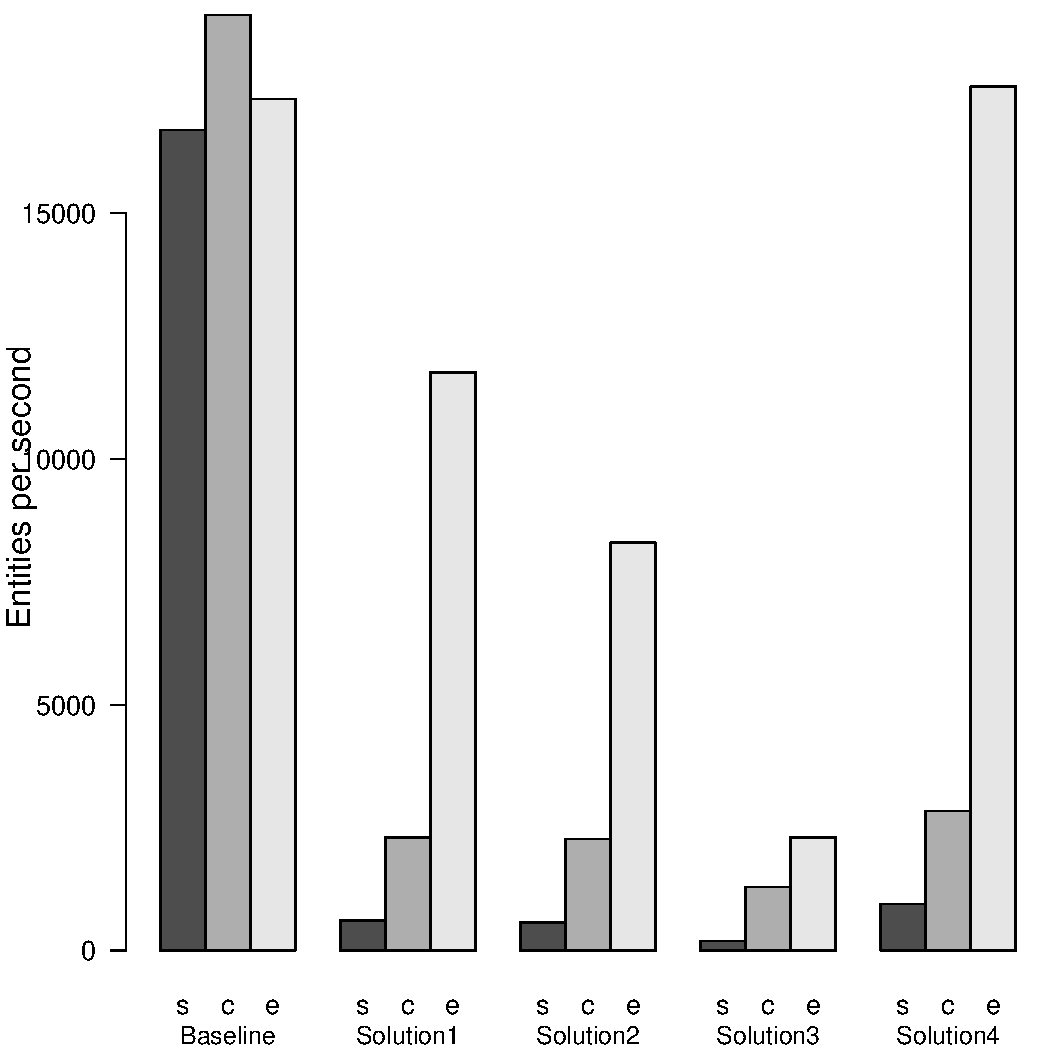
\includegraphics[width=\W]{figure/result/barplot-delete-tp.pdf} \label{fres:delete-}\label{fres:Delete-throughput}}
		\caption{Performance of Solutions in Update}\label{fres:Delete}
	\end{figure}
 
As seen in  the results, the \texttt{delete} in \texttt{Enrolment}
is the fastest in all the solutions, while  \texttt{delete} in
\texttt{Student} is the slowest. The \texttt{delete} operation on 
\texttt{Course} is faster than deleting \texttt{Student} entities but it
always takes more time than \texttt{delete} in \texttt{Enrolment}.

As seen in \texttt{update}, the difference in  performance of the operation
on the different entities is because of the referential integrity rules on
child and parent entities. Deleting \texttt{Enrolment} entities is faster as it 
does not invoke any referential integrity validations since \texttt{Enrolment}
has no child dependencies in it.
However, this operation is  slower than the baseline in all the solutions
because it involves accessing metadata to retrieve the relevant constraints of
\texttt{Enrolment} in order to determine if any child dependencies exist or
not.

Deleting \texttt{Student} entities is a cascaded operation which involves
deleting the child dependencies in the \texttt{Enrolment} column family. This
operation is slower because  the relevant constraints need to be  accessed and
the child entities in \texttt{Enrolment}  that have a reference to the
\texttt{Student} have to be deleted. 

Similarly, \texttt{delete} on \texttt{Course} entities also involves accessing
the relevant constraints and finding the child dependencies in
\texttt{Enrolment}. However, in the experiments,  all the entities in
\texttt{Enrolment} are already deleted before \texttt{delete} is invoked on
\texttt{Course} entities. Hence, \texttt{delete} in \texttt{Course} actually
deletes the entities as there are no existing child dependencies.
Notice that \texttt{delete} on \texttt{Course} involves the time to access
metadata as well as \texttt{Enrolment} in order to search for any existing child
dependencies and values are deleted from a single column family. However,
\texttt{delete} on \texttt{Student} entities involve deleting values from two
column families (\texttt{Student} and \texttt{Enrolment}). This
makes \texttt{delete} in \texttt{Course} faster than \texttt{delete} in
\texttt{Student}.

Finally, Figures~\ref{fres:delete-response-time}
and~\ref{fres:delete-throughput} show the average response time and throughput
of \texttt{delete} on all the entities. It can be seen from these results that
Solution~4 takes the least time to complete a \texttt{delete} operation on each
entity, while Solution~3 takes the most time. Since Solution~4 caches the
metadata of all the entities, it avoids multiple accesses to the
\texttt{Metadata} column family whereas Solution~3 requires accessing
\texttt{Metadata} each time a constraint has to be accessed for an entity. The
performance of Solutions~1 and 2 are comparable to each other even though
Solution~2 takes slightly more time due to its additional search operation to
locate the top row.

When compared to the baseline, all the solutions take longer to delete entities.
As mentioned previously, this is because all the solutions involve accessing
relevant constraints and performing validations.
Solutions~1 and 2 are almost 2 times slower than baseline  when
\texttt{Enrolment} entities are deleted while Solution~3 is almost 7 times
slower. Solution~4 is almost similar to the baseline in this case  which shows
that accessing the metadata does not cause much difference in the performance.


However, in a cascaded delete which includes referential integrity validations
Solutions~1 and 2 are more than 23 times slower than the
baseline while Solution~3 is almost 80
times slower. Solution~4  is up to 17 times slower than the baseline.



\begin{landscape}
		\begin{figure}
		\centering
		\newcommand{\W}{.4\textwidth}
			\subfigure[Delete on Student]
			{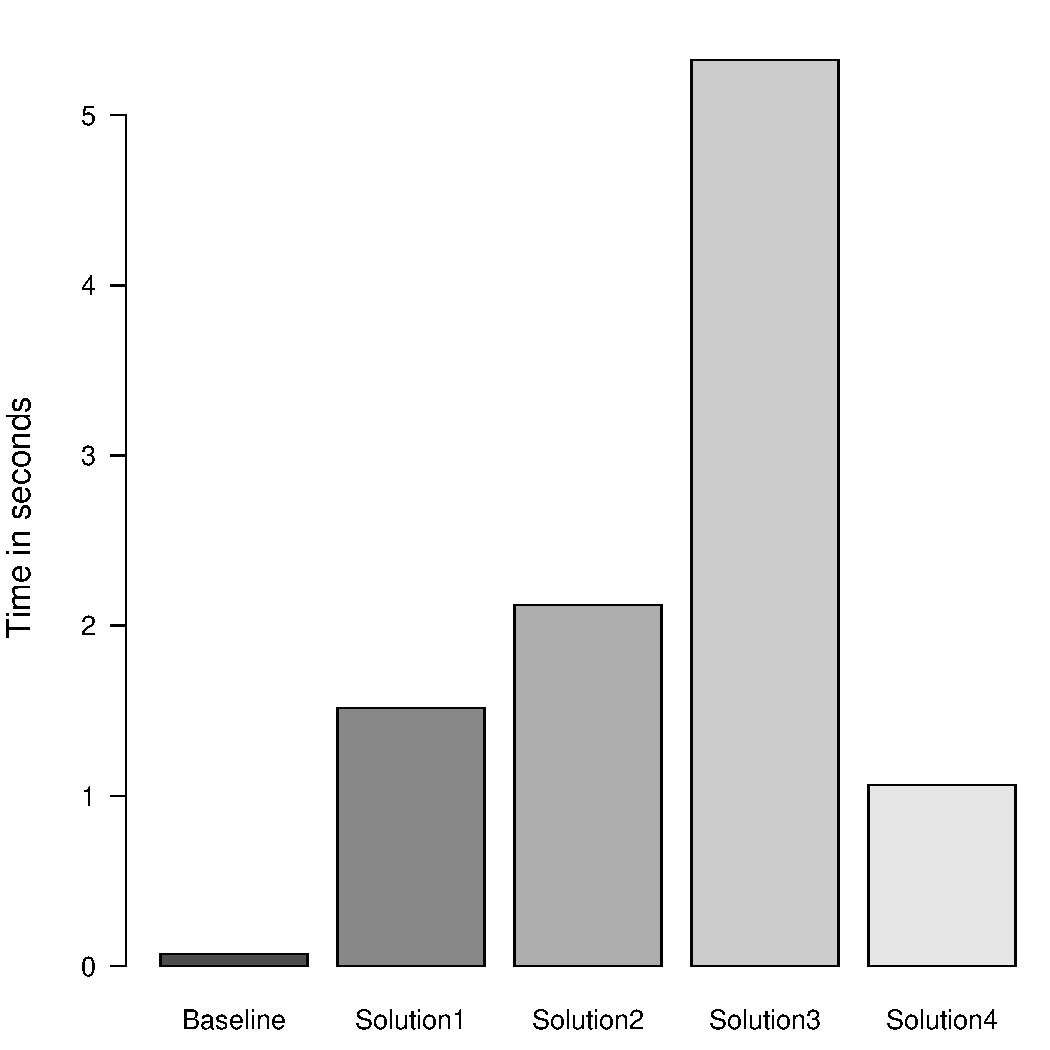
\includegraphics[width=\W]{figure/result/barplot-delete_student-rt.pdf}
			\label{fres:delete-user}}
			\subfigure[Delete on Course]
			{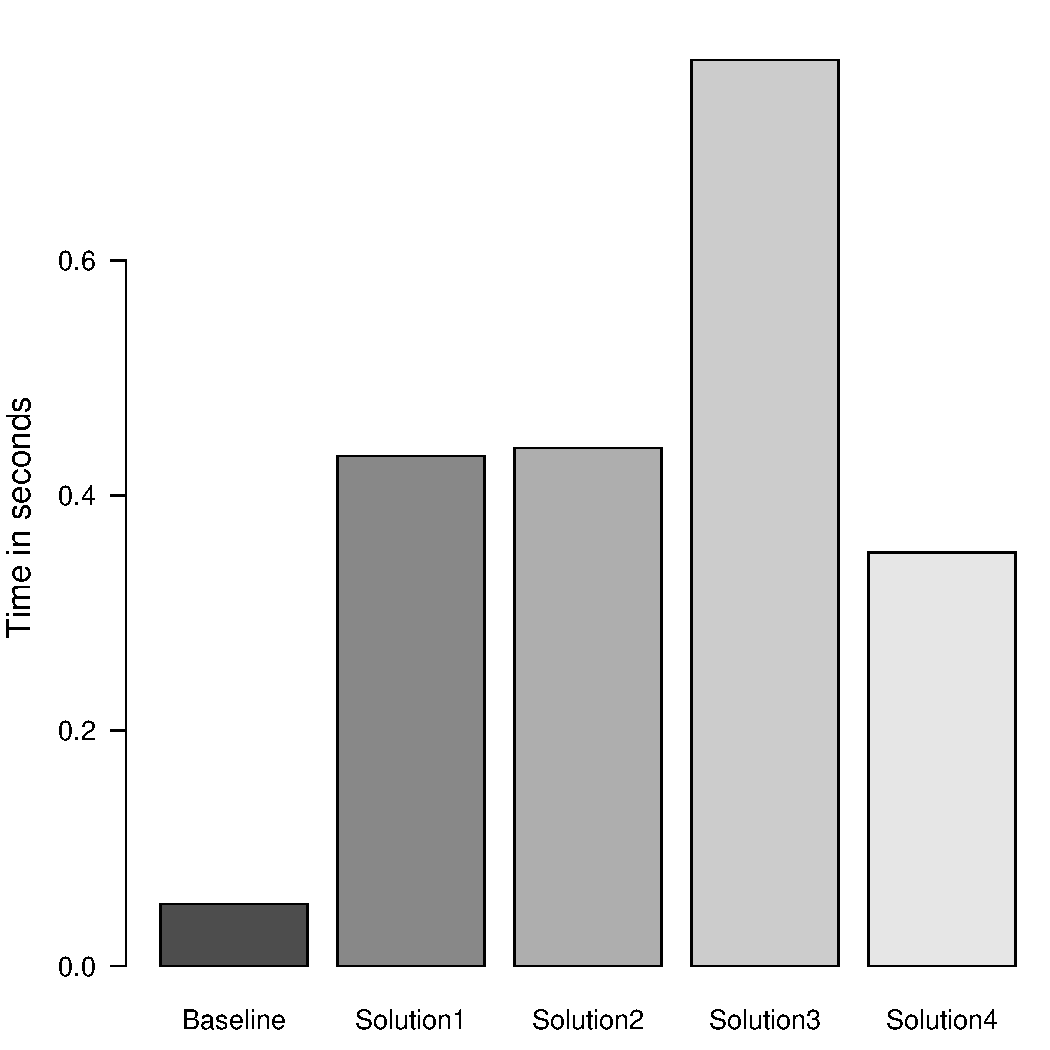
\includegraphics[width=\W]{figure/result/barplot-delete_course-rt.pdf}
			\label{fres:delete-course}}
			\subfigure[ Delete on Enrolment ]
			{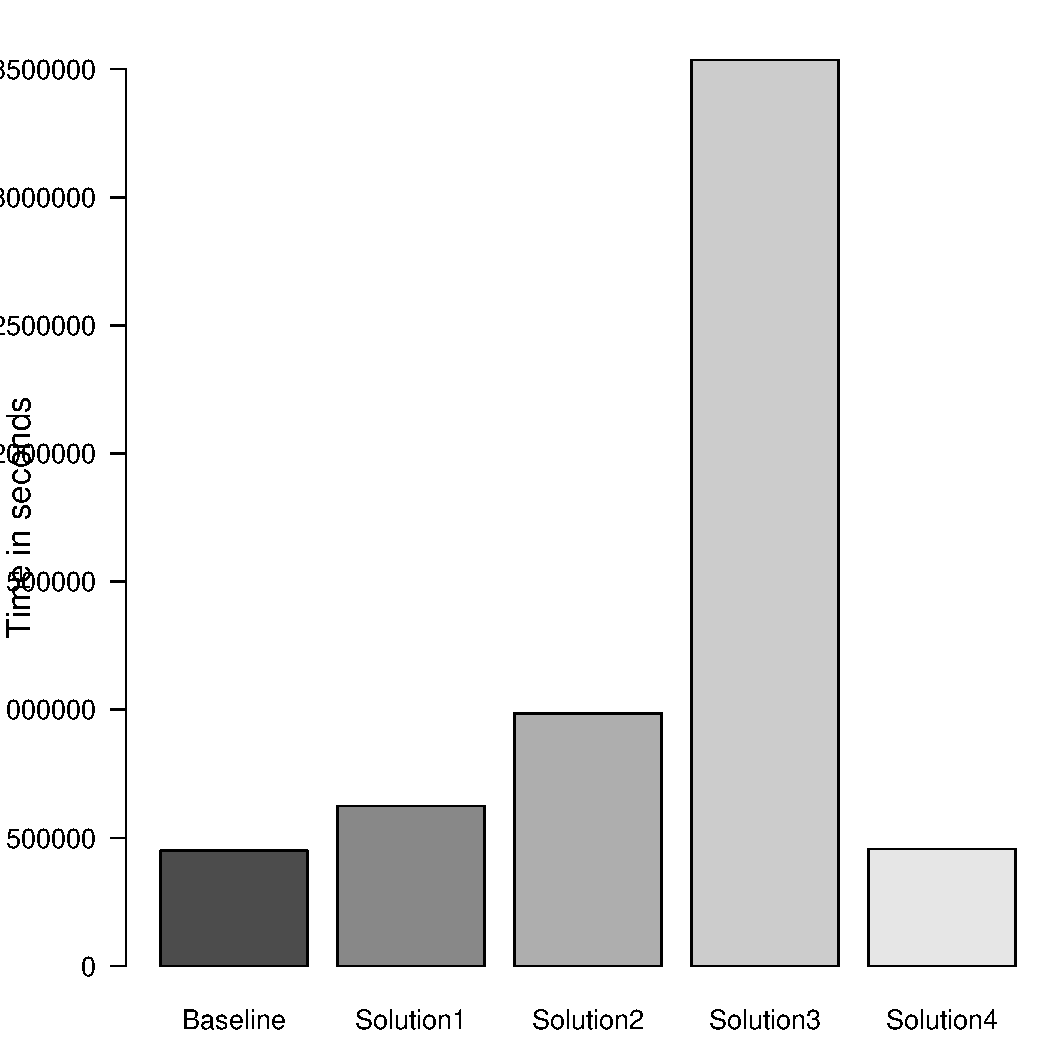
\includegraphics[width=\W]{figure/result/barplot-delete_enrolment-rt.pdf}
			\label{fres:delete-enrolment}}
			\caption{Response time deleting entities}\label{fres:delete-response-time}
						
			\subfigure[Delete on Student]
			{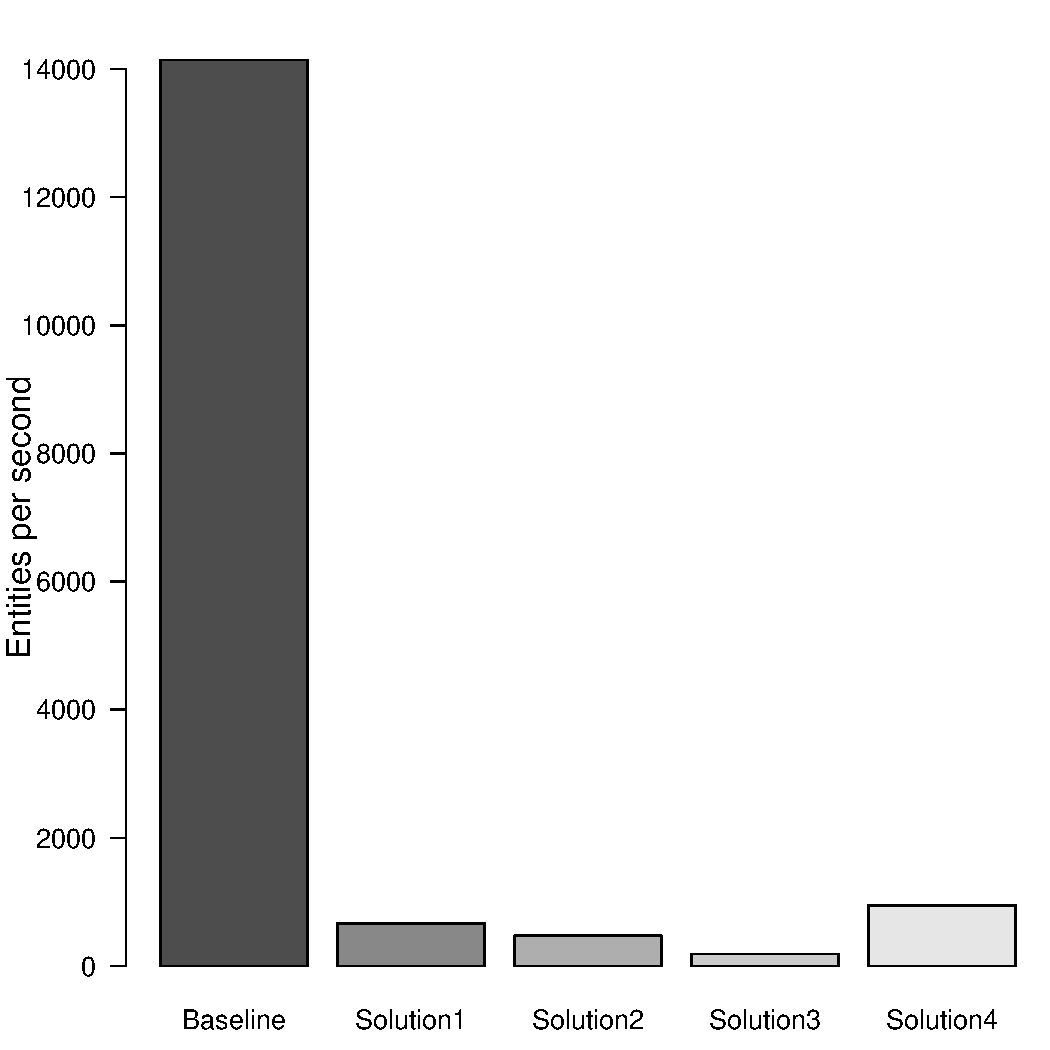
\includegraphics[width=\W]{figure/result/barplot-delete_student-tp.pdf} \label{fres:delete-}}
			\subfigure[Delete on Course]
			{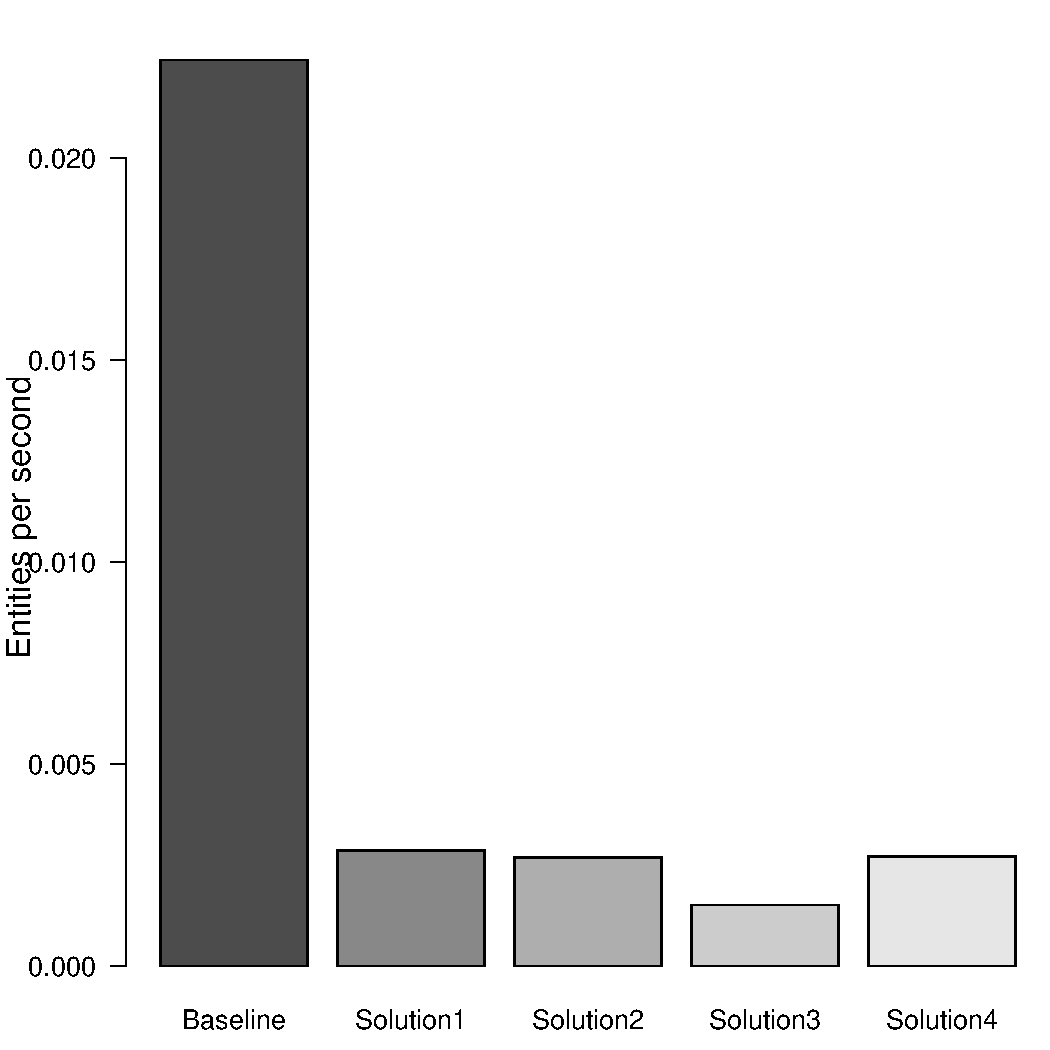
\includegraphics[width=\W]{figure/result/barplot-delete_course-tp.pdf} \label{fres:delete-}}
			\subfigure[Delete on Enrolment]
			{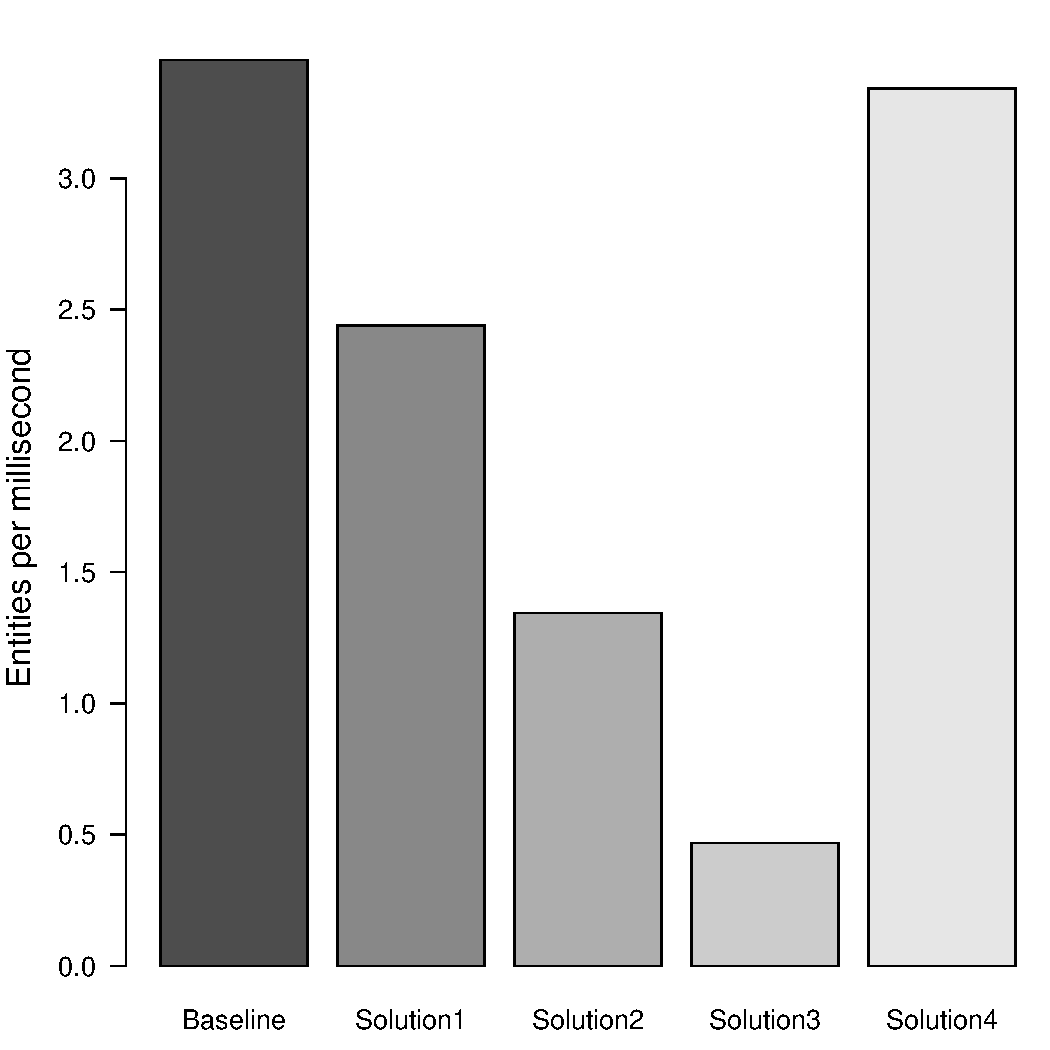
\includegraphics[width=\W]{figure/result/barplot-delete_enrolment-tp.pdf} \label{fres:delete-}}
			\caption{Throughput deleting entities}\label{fres:delete-throughput}
		\end{figure}
\end{landscape}


% Moreover,   when the experiments are run \texttt{insert} on these entities are
% the first operations to take place and the results can be slightly influenced
% by the initialisation of the column families and the keyspace.   However,   the
% difference is small and only a fraction of a millisecond. 
% the number  of columns that are updated in \texttt{Enrolment} is much lesser
% than the other column families.   This means that \texttt{update} on
% \texttt{Enrolment} involves fewer search by indexes and writes for the new
% values,   to be precise it involves only three searches and writes to update
% its three columns.    On the other hand,  \texttt{Student} and \texttt{Course}
% column families have more number of columns to be updated in each
% \texttt{update} operation. 

\section{Comparison of the Operations} \label{s:comparisonOfOperations}
 
In order to compare the operations,  their performance  is grouped by solutions
and presented in Figures~\ref{fres:ResponseTimeOfSolutions}
and~\ref{fres:ThroughputOfSolutions}. 
Generally,  the \texttt{insert} operation takes the least time across the
solutions as it does not involve any cascaded operations and referential
integrity constraints have to be satisfied only for the child entities.  This
involves ensuring the existence of foreign keys as primary keys in the parent
column families and then inserting the child entities into their respective
column families. 

On the other hand,   the \texttt{update} operation takes the most time  in every
solution,   mainly due to its cascaded behaviour on parent entities,   which
involves changing the parent primary key,   accessing child column families and
changing its foreign key values.  Note that \texttt{update} on \texttt{Enrolment}
is similar to \texttt{insert} on \texttt{Enrolment} across the solutions, 
because both operations involve checking whether the foreign keys exist in the
parent column families and inserting the values only in \texttt{Enrolment}. 
On the other hand,   \texttt{update} on parent entities (\texttt{Student} and
\texttt{Course})  take more time than inserting parent entities because
\texttt{update} involves additional searches and operations (\texttt{insert} and
\texttt{delete}) in both the parent and child column families. 

The \texttt{delete} operation is slower than the \texttt{insert} in the case of
parent entities and faster than \texttt{insert} in the case of child entities. 
This is because  referential integrity constraints have to be satisfied only in
the case of the  parent entities for this operation. 
% However,  inserting child entities require referential integrity constraints to
% be satisifed which makes \texttt{delete} faster than \texttt{insert} in the
% case of child entities. 
When \texttt{delete} and \texttt{update} operations are compared,  it can be seen
that the ratio of their performances  on the entities are similar,  which is
because both these operations are cascaded on parent entities. 
For example,  \texttt{update} on \texttt{Student} takes the most time amongst
entities,  and similarly,  \texttt{delete} on \texttt{Student} takes the most time
amongst the entities.  However,  in general,  deleting entities is faster than
updating them.  This is because updating entities involves more operations as
both \texttt{insert} and \texttt{delete} are performed on  child and
parent column families,  while deleting entities involves inserting empty values
in the place of the entity attributes to mark them as deleted (tombstone
effect).  Moreover,  in \texttt{update},  referential integrity constraints
have to satisfied for both parent and child entities,  but in
\texttt{delete},  these have to be satisfied only for the parent entities. 

Further information about the results for the operations and solutions are
provided in Appendices~\ref{apx:insert},  \ref{apx:update},  and
~\ref{apx:delete}. 


% Conversely,  deleting child entities is faster than inserting child entities
% because referential integrity constraints. 
%  
%  inserting parent entities do not cause referential integrity validations,   but
%  deleting them does.   Conversely,   deleting child entities is faster than
% inserting child entities since it does not trigger such validations. 

% 
% Across all solutions,  the \texttt{insert}
% operation is the one that has best performance when it comes to \texttt{Student}
% and \texttt{Course} as these entities do not have referential integrity
% constraints to be satisfied.  Such is not the case for \texttt{Enrolment}
% entities as these have foreign key values that reference entities in
% \texttt{Student} and \texttt{Course}.  Hence,  the referential integrity
% validation ensures that 
% 
% 
% 
% From these figures it can be seen that the
% \texttt{insert} operation  takes the least time to complete when compared
% to \texttt{update} and \texttt{delete} operations.   This is mainly because in
% \texttt{insert},  validations are triggered on only the \texttt{Enrolment} column
% family. 
% 
% On the other hand,   the \texttt{update} operation takes the most time  in every
% solution,   mainly due to its cascaded behaviour on parent entities,   which
% involves changing the parent primary key,   accessing child column families and
% changing its foreign key values. 
% Note that \texttt{update} on \texttt{Enrolment} is similar to \texttt{insert} on
% \texttt{Enrolment} because both operations involve checking whether the foreign
% keys exist in the parent column families and inserting the values only in
% \texttt{Enrolment}. 
% However,   \texttt{update} on \texttt{Student} and  \texttt{Course} entities take
% more time than inserting students and courses because \texttt{update} involves
% additional searches and operations (\texttt{insert} and \texttt{delete})
% in more than one column family.  
% 
% The \texttt{delete} operation is faster than \texttt{update} in all the
% solutions since entities are not immediately deleted due to the tombstone
% paradigm in Cassandra.   Moreover,  it involves only a single operation
% unlike the \texttt{update} operation which causes both an \texttt{insert} and a
%  \texttt{delete}.   Moreover,  deleting child entities do not cause validations
%  but updating any entity causes validations. 

% When compared with the \texttt{insert} operation,   \texttt{delete} is slower in
% the case of parent entities,   \texttt{Student} and \texttt{Course}.   This is
% because inserting parent entities do not cause referential integrity
% validations,   but deleting them does.   Conversely,   deleting child entities is
% faster than inserting child entities since it does not trigger such validations. 


\begin{landscape}

		\begin{figure}
		\newcommand{\W}{.345\textwidth}
		\centering
			\subfigure[Solution 1]
			{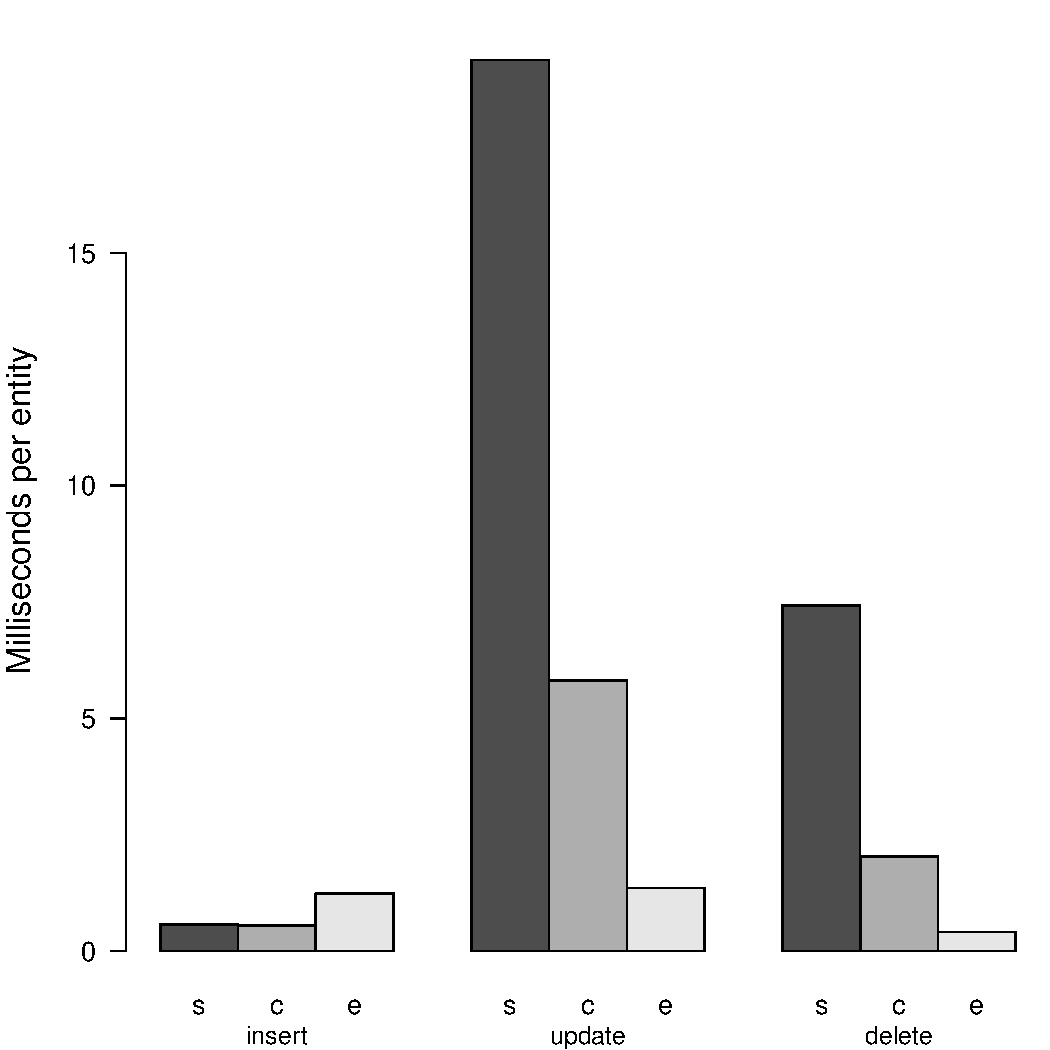
\includegraphics[width=\W]{figure/result/barplot-Solution1-rt.pdf}
			\label{fres:Summary-Solution1}}
			\subfigure[Solution 2]
			{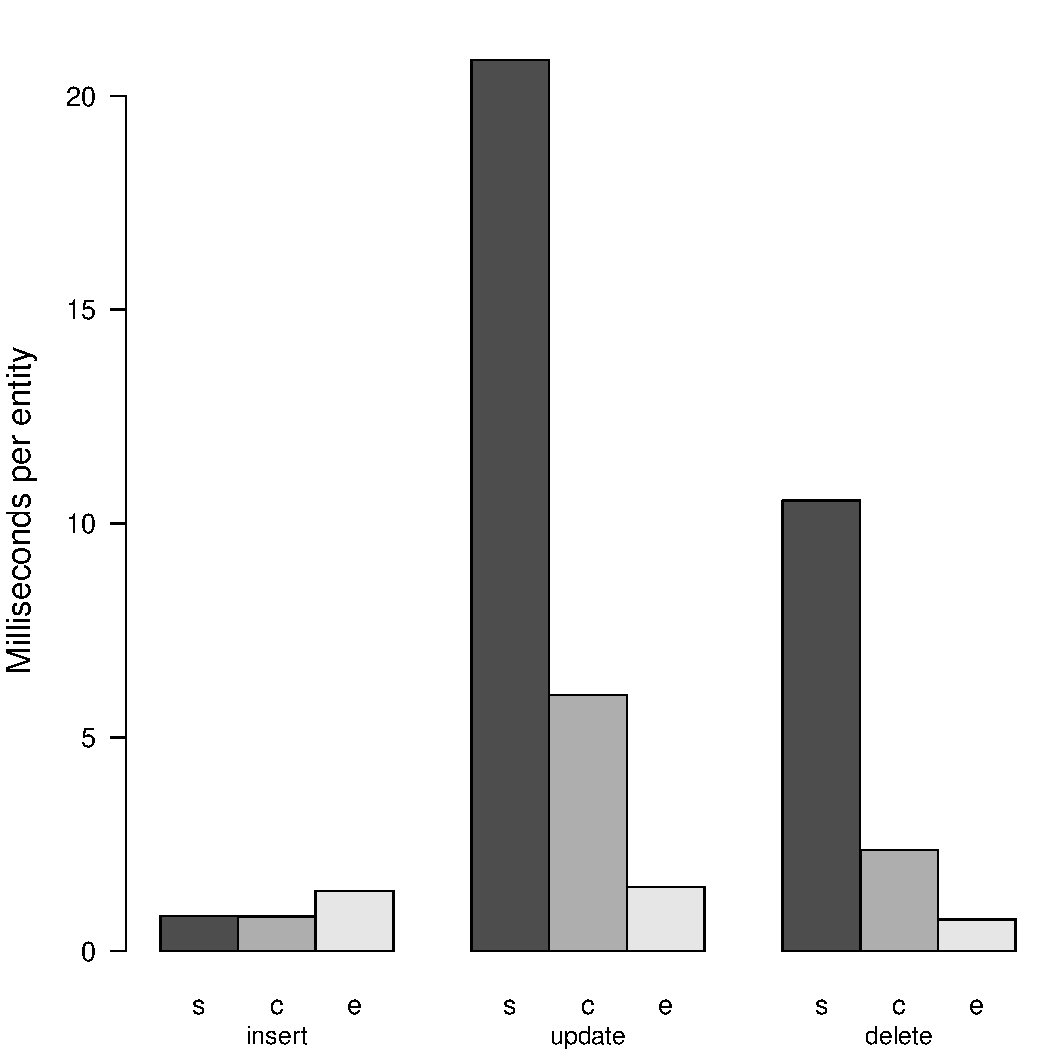
\includegraphics[width=\W]{figure/result/barplot-Solution2-rt.pdf}
			\label{fres:Summary-Solution2}}
			\subfigure[Solution 3]
			{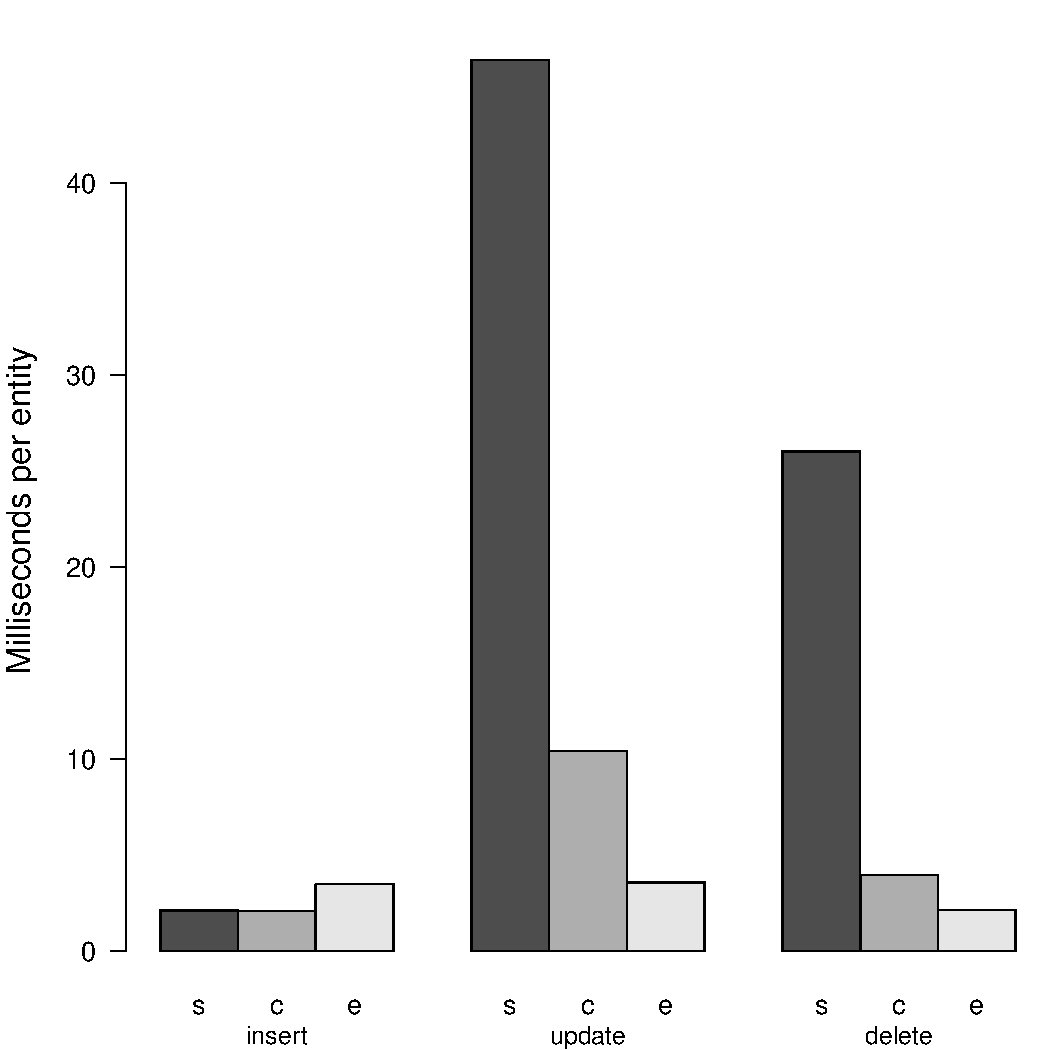
\includegraphics[width=\W]{figure/result/barplot-Solution3-rt.pdf}
			\label{fres:Summary-Solution3}}
			\subfigure[Solution 4]
			{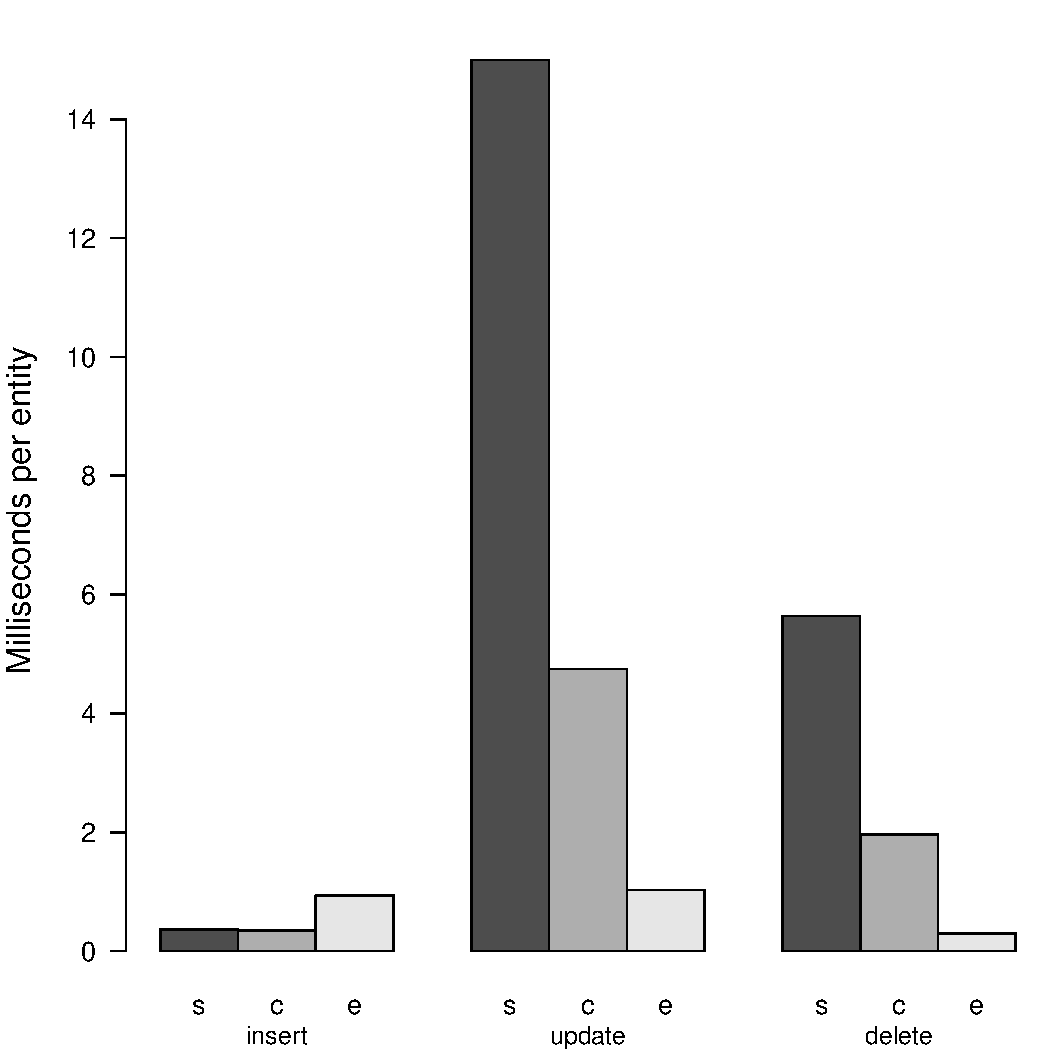
\includegraphics[width=\W]{figure/result/barplot-Solution4-rt.pdf}
			\label{fres:Summary-Solution4}}
			\captionof{figure}{Response Time of the
			Solutions}\label{fres:ResponseTimeOfSolutions}
			
			\subfigure[Solution 1]
			{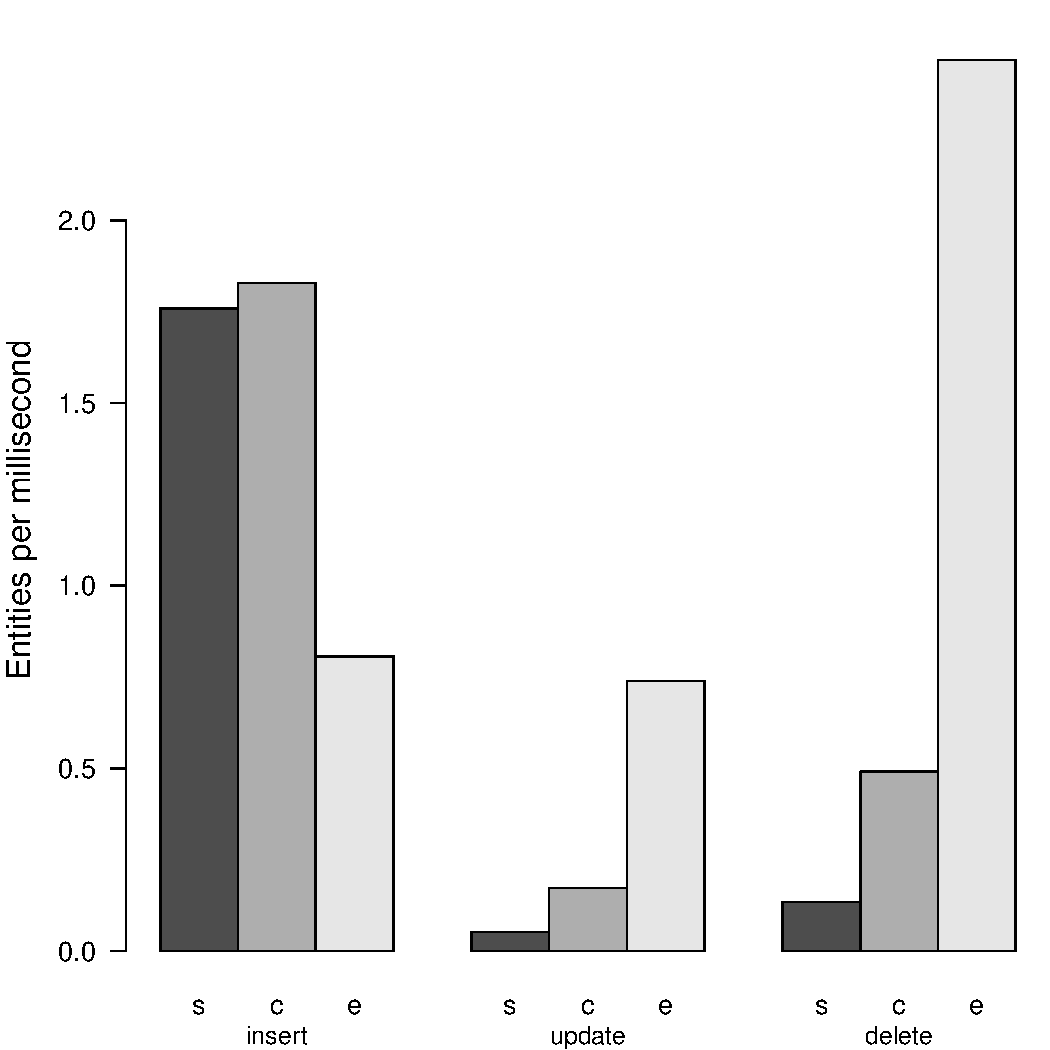
\includegraphics[width=\W]{figure/result/barplot-Solution1-tp.pdf}
			\label{fres:Summary-Solution1}}
			\subfigure[Solution 2]
			{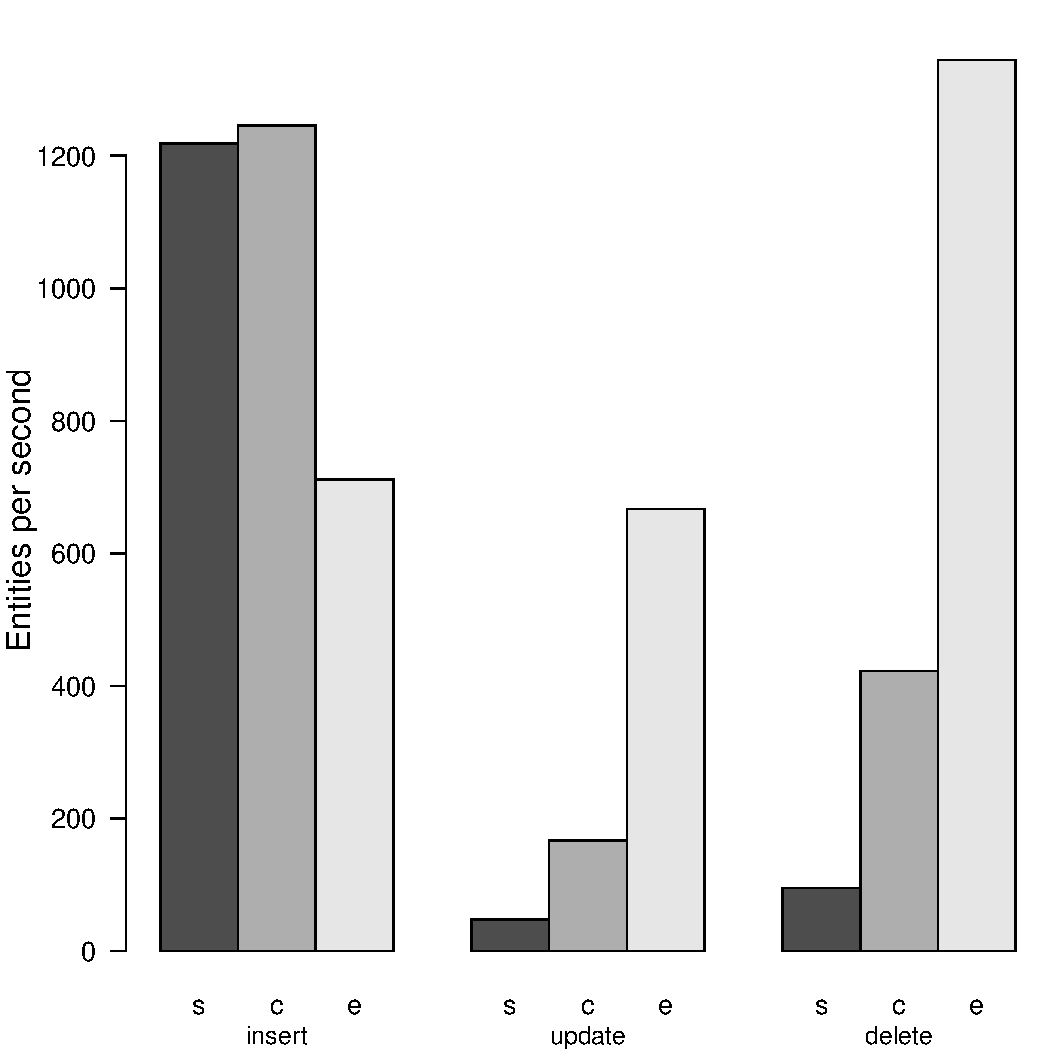
\includegraphics[width=\W]{figure/result/barplot-Solution2-tp.pdf}
			\label{fres:Summary-Solution2}}
			\subfigure[ Solution 3]
			{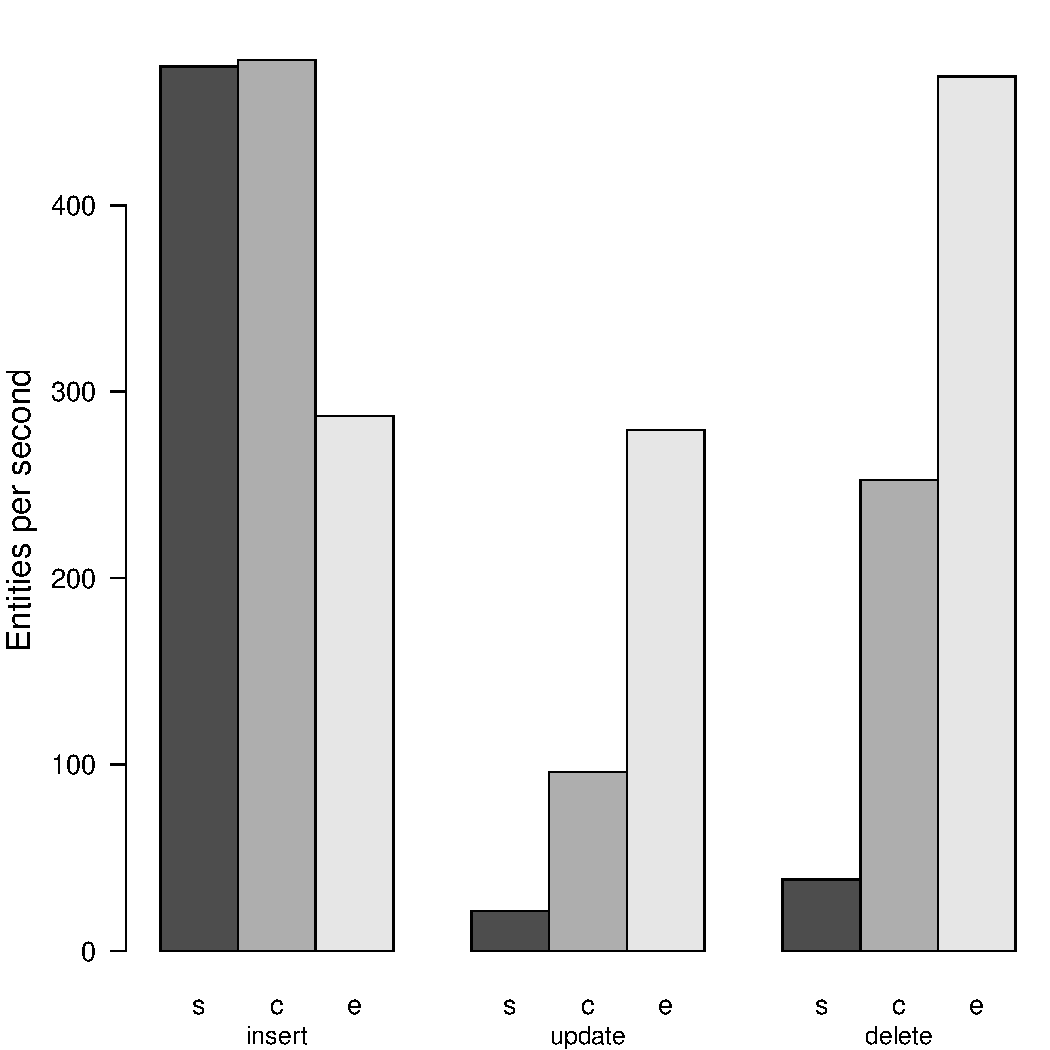
\includegraphics[width=\W]{figure/result/barplot-Solution3-tp.pdf}
			\label{fres:Summary-Solution3}}
			\subfigure[ Solution 4]
			{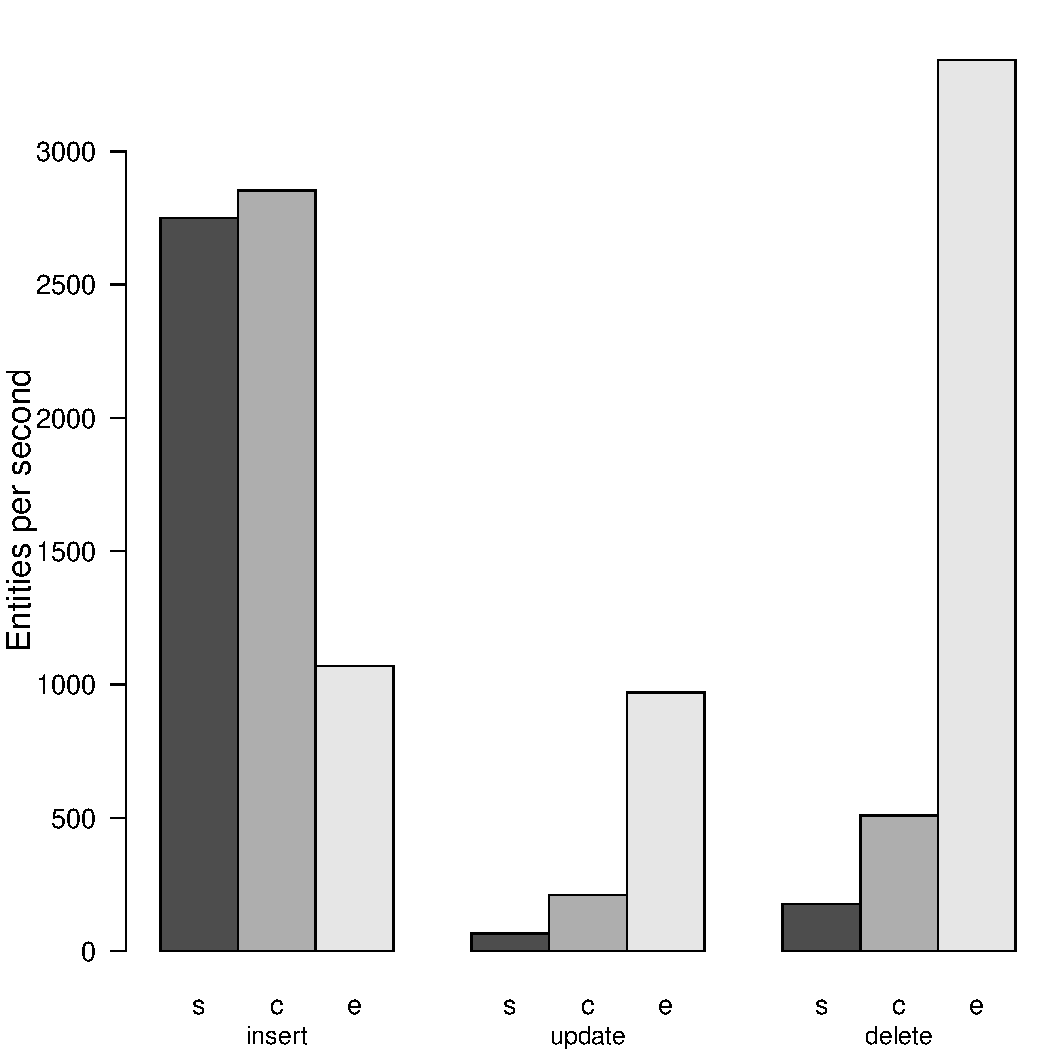
\includegraphics[width=\W]{figure/result/barplot-Solution4-tp.pdf}
			\label{fres:Summary-Solution4}}
			\caption{Throughput of the Solutions}\label{fres:ThroughputOfSolutions}
		\end{figure}
\end{landscape}


\section{Summary} \label{s:results-summary}

This chapter presented the results and discussions from the experiments designed
to evaluate the performance of the different \ac{CRUD} operations under
different referential integrity constraints in each of the solutions.
The results were assessed in terms of the average response time and throughput
of each operation. The results reflected that Solution~4 performs the best
amongst the solutions, and performs similar to the baseline when no referential
integrity constraints need to be satisfied (e.g. inserting parent entities),
because it caches the metadata and re-uses it to avoid multiple access to the
\texttt{Metadata} column family.
Solution~3 performs the worst amongst all and is slower than the baseline even
when no referential integrity constraints need to be satisfied because
simply accessing the metadata from a separate column family each time affects
its performance.
Solutions~1 and 2 perform similarly in all the operations on the entities which
is mainly because the metadata is embedded with the actual data.   Solution~2
consumes slightly more time than Solution~1 as it searches for the top row to
identify constraints on each operation.

The results showed that amongst the operations,   \texttt{insert} took the least
time while \texttt{update} took the most time,   and \texttt{delete} was faster
than \texttt{insert} only in the case of child entities.   These variations were
mainly due to the different referential integrity rules that are applied on
parent and child entities,   especially because of the \texttt{DeleteRule}
applied on these entities.  

The entities required different behaviours in each operation due to the various
referential integrity rules as well as  the data manipulation rules applied on
them.
\texttt{Enrolment} entities required to satify referential integrity constraints
during \texttt{insert} and \texttt{update} operations as it is a child entity,
while \texttt{Student} and \texttt{Course} are parent entities and required to
satisfy these constraints in both \texttt{update} and \texttt{delete}.   Thus,
parent entities are faster to operate upon in an \texttt{insert} operation,  
while child entities are faster only in a \texttt{delete} operation.
	
